% For copyright and license information, see uiucthesis2021.dtx and derivatives.
\documentclass{uiucthesis2021}
\usepackage[utf8]{inputenc}
\usepackage[english]{babel}
\usepackage{csquotes}
\usepackage{microtype}
\usepackage{listings}
\usepackage{amsmath,amsthm,amssymb}
\usepackage{minted}
\usepackage{relsize}
\usepackage[normalem]{ulem}
\usepackage{pifont}
\newcommand{\cmark}{\ding{51}}%
\newcommand{\xmark}{\ding{55}}%
\usepackage[bookmarksdepth=3,linktoc=all,colorlinks=true,urlcolor=blue,linkcolor=black,citecolor=black]{hyperref}
\usepackage[capitalize]{cleveref}
\usepackage[citestyle=numeric-comp, bibstyle=ieee, backend=biber, eprint=false]{biblatex}

\usepackage{lipsum}  % just for placeholder code

% \usepackage[acronym,toc]{glossaries}
\setcounter{tocdepth}{2}
\usepackage[printonlyused,withpage]{acronym}
% \acro{esom}[ESOM]{energy system optimization model}
\acrodefplural{esom}[ESOMs]{energy system optimization models}
\acro{lp}[LP]{linear programming}
\acrodefplural{lp}[LPs]{linear programs}
\acro{eroi}[EROI]{energy return on investment}
\acro{milp}[MILP]{mixed-integer linear programming}
\acrodefplural{milp}[MILPs]{mixed-integer linear programs}
\acro{osier}[\texttt{Osier}]{Open-source multi-objective energy system framework}
\acro{dapl}[DAPL]{Dakota Access Pipeline}
\acro{temoa}[\texttt{Temoa}]{Tools for Energy Model Optimization and Analysis}
\acro{pygen}[\texttt{PyGenesys}]{Python for Generating Energy Systems}
\acro{pymoo}[\texttt{Pymoo}]{Multi-Objective Optimization in Python}
\acro{pyomo}[\texttt{Pyomo}]{Python-based, open-source optimization modeling language}
\acro{hsj}[HSJ]{Hop-Skip-Jump algorithm}
\acro{mga}[MGA]{Modeling-to-Generate-Alternatives}
\acro{moo}[MOO]{multi-objective optimization}
\acro{ghg}[GHG]{greenhouse gas}
\acrodefplural{ghg}[GHGs]{greenhouse gases}
\acro{sp}[SP]{stochastic programming}
\acro{mc}[MC]{Monte Carlo}
\acro{pa}[PA]{parametric analysis}
\acro{nsga2}[NSGA-II]{Non-Dominated Sorting Genetic Algorithm-II}
\acro{nsga3}[NSGA-III]{Non-Dominated Sorting Genetic Algorithm-III}
\acro{unsga3}[UNSGA-III]{Unified Non-Dominated Sorting Genetic Algorithm}
\acro{ga}[GA]{genetic algorithm}
\acrodefplural{ga}[GAs]{genetic algorithms}
\acro{ws}[WS]{weighted-sum}
\acro{ec}[EC]{$\epsilon$-constraint}
\acro{vre}[VRE]{variable renewable energy}
\acro{nrc}[NRC]{Nuclear Regulatory Commission}
\acro{nrel}[NREL]{National Renewable Energy Laboratory}
\acro{atb}[ATB]{Annual Technology Baseline}
\acro{stm}[STM]{social transition movement}
\acro{ccs}[CCS]{carbon capture and storage}
\acro{pve}[PVE]{participatory value evaluation}
\acro{ipcc}[IPCC]{International Panel on Climate Change}
\acro{un}[UN]{United Nations}
\acro{gva}[GVA]{gross value added}
\acro{gdp}[GDP]{gross domestic product}
\acro{wtp}[WTP]{willingness to pay}
\acro{wpe}[WPE]{weighted permutation entropy}
\acro{igdp}[IGD+]{inverted generational distance plus}
\acro{icap}[iCAP]{Illinois Climate Action Plan}
\acro{isee}[iSEE]{Institute for Sustainability, Energy, and Environment}
\acro{ipcc}[IPCC]{International Panel on Climate Change}
\acro{deap}[\texttt{DEAP}]{Deep Evolutionary Algorithms in Python}
\acro{uiuc}[UIUC]{University of Illinois Urbana-Champaign}
\acro{pcp}[PCP]{parallel coordinate plot}
\acro{nimby}[NIMBY]{not-in-my-backyard}
\acro{nimbyism}[NIMBYism]{not-in-my-backyard}
\acro{snf}[SNF]{spent-nuclear-fuel}
\acro{smr}[SMR]{small modular reactor}
\acrodefplural{smr}[SMRs]{small modular reactors}
\acro{ipa}[IPA]{Illinois Power Agency}
\acro{icc}[ICC]{Illinois Commerce Commission}
\acro{set}[SET tool]{Screening and Evaluation Tool}
\acro{mca}[MCA]{municipal choice aggregation}
\acro{imea}[IMEA]{Illinois Municipal Electric Agency}
\acro{ppa}[PPA]{power purchase agreement}
\acro{pypsa}[\texttt{PyPSA}]{Python for Power Systems Analysis}
\acro{lib}[LiB]{lithium-ion battery}
\acrodefplural{lib}[LiBs]{lithium-ion batteries}
\acro{reason}[RE$^3$ASON]{Renewable Energies and Energy Efficiency Analysis and System Optimization}
\acro{mavt}[MAVT]{multi-attribute value theory}
\acro{mcda}[MCDA]{multi-criteria decision analysis}
\acro{ngo}[NGO]{non-governmental organization}
\acro{co2}[CO$_2$]{carbon dioxide}
\acro{co2eq}[CO$_2$-eq]{CO$_2$-equivalent}

\usepackage{float}
\usepackage{placeins}
\usepackage{booktabs}
\usepackage{colortbl}
\usepackage{xltabular}
\usepackage{multirow}
\usepackage{caption}
\usepackage{subcaption}
\usepackage{graphics}
\usepackage{graphicx}
\usepackage{tikz}
\usepackage{pgfplots}
\usepackage{rotating}
\usepackage{xcolor}
\usepackage[most]{tcolorbox}
\usepackage{bibentry}
\nobibliography*

\definecolor{LightGray}{gray}{0.9}
\definecolor{illiniblue}{HTML}{B1C6E2}
\definecolor{illiniorange}{HTML}{f8c2a2}
\graphicspath{figures/}

\newcommand{\mathdefault}[1][]{}

\newtcolorbox{noteBox}[1][]{
    width=\textwidth,
    fonttitle=\bfseries,
    breakable,
    fonttitle=\bfseries\color{Black},
    colframe=illiniblue,
    colback=illiniblue!10
    #1}

\usetikzlibrary{positioning, arrows, decorations, shapes}
\usetikzlibrary{shapes.geometric,arrows}

\def\checkmark{\tikz\fill[scale=0.4](0,.35) -- (.25,0) -- (1,.7) -- (.25,.15) -- cycle;} 
\tikzstyle{loblock} = [rectangle, draw, fill=illiniorange, 
text width=15em, text centered, rounded corners, minimum height=3em]
\tikzstyle{lbblock} = [rectangle, draw, fill=illiniblue, 
text width=15em, text centered, rounded corners, minimum height=3em]
\tikzstyle{oblock} = [rectangle, draw, fill=illiniorange, 
text width=10em, text centered, rounded corners, minimum height=3em]
\tikzstyle{bblock} = [rectangle, draw, fill=illiniblue, 
text width=10em, text centered, rounded corners, minimum height=3em]
\tikzstyle{arrow} = [thick,->,>=stealth]
\tikzstyle{bbblock} = [rectangle, draw, fill=illiniblue, 
text width=1em, text centered, rounded corners, minimum height=1em]
\tikzstyle{boblock} = [rectangle, draw, fill=illiniorange, 
text width=1em, text centered, rounded corners, minimum height=1em]
\tikzstyle{e72block} = [rectangle, fill=none, 
text width=7.3em, text centered, rounded corners, minimum height=2em]
\tikzstyle{o72block} = [rectangle, draw, fill=illiniorange, 
text width=7.3em, text centered, rounded corners, minimum height=2em]
\tikzstyle{p72block} = [rectangle, draw, fill=purple, 
text width=7.3em, text centered, rounded corners, minimum height=2em]
\tikzstyle{g72block} = [rectangle, draw, fill=green, 
text width=7.3em, text centered, rounded corners, minimum height=2em]
\tikzstyle{b72block} = [rectangle, draw, fill=illiniblue, 
text width=7.3em, text centered, rounded corners, minimum height=2em]
\tikzstyle{e82block} = [rectangle, fill=none, 
text width=8.3em, text centered, rounded corners, minimum height=2em]
\tikzstyle{e92block} = [rectangle, fill=none, 
text width=9.3em, text centered, rounded corners, minimum height=2em]
\tikzstyle{b82block} = [rectangle, draw, fill=illiniblue, 
text width=8em, text centered, rounded corners, minimum height=2em]
\tikzstyle{b223block} = [rectangle, draw, fill=illiniblue, 
text width=22em, text centered, rounded corners, minimum height=3em]

% uncomment the below to show a grid on all pages
% \usepackage[grid, gridunit=in, gridcolor=blue!40, subgridcolor=blue!20]{eso-pic}

\addbibresource{2025-dotson-phd.bib}

\newcounter{counterforappendices}

\begin{document}

\title{Towards a Holistic Integration of Energy Justice and Energy System Engineering}
\author{Samuel G. Dotson}
\department{Nuclear, Plasma, and Radiological Engineering}
% \concentration{}
\phdthesis
\degreeyear{2025}
\committee{
    Associate Professor Kathryn D. Huff, Co-Chair\\
    Assistant Professor Madicken Munk, Co-Chair\\
    Professor James F. Stubbins\\
    Professor Clifford Singer\\
    Assistant Professor McKenzie F. Johnson\\
    Research Scientist, Denia Djoki\'c}
\maketitle

\frontmatter

\begin{abstract}
    Solving climate change will require our globalized society to transition from
fossil fuel infrastructure to clean energy infrastructure. This transition must
also be done equitably and justly to prevent entrenching further injustices to
marginalized and vulnerable communities. To that end, this thesis develops the
first multi-objective energy system optimization framework, \texttt{Osier}, to
enhance the democratic engagement necessary for a just transition. Rather than
making projections about the future, \texttt{Osier} accomplishes this goal by
combining user-supplied energy demand data with technology-specific data (e.g.,
emissions, land-use, cost) and delivers a set of co-optimal energy systems
(i.e., capacities for different energy generating technologies) that balance
competing priorities (e.g., emissions, cost, or land-use). Further,
\texttt{Osier} acknowledges structural uncertainty --- the existence of
unmodeled or \textit{unmodelable} objectives --- by extending the conventional
modeling-to-generate-alternatives approach into N-dimensional objective space.
This approach does not promise to model the unmodelable, rather it recognizes
that any presentation of ``optimal'' solutions will necessarily miss these
unmodelable priorities and that interesting solutions may be contained in a
models sub-optimal space.

This thesis verified \texttt{Osier}'s suitability for energy modeling problems
with several \textit{in silico} experiments. The first set of experiments
establish \texttt{Osier}'s superiority at exploring decision space over the
mature \texttt{Temoa} framework. A second set of experiments demonstrates
\texttt{Osier} on relevant problems, such as deciding among many nuclear fuel
cycle options. Finally, this thesis presents the results of thirteen expert
interviews which support \texttt{Osier}'s utility for facilitating democratic
engagement between decision makers and their constituents, thereby attending
to issues related to procedural and recognition justice.
\end{abstract}

% \begin{dedication}
% [F]or the kids like me who got ADHD.\\
% \rule{17em}{0.4pt}\\
% \hspace{13em} ``ISIS''\\
% % \hspace{8em} --- Joyner Lucas\\ 
% \hspace{10em} Joyner Lucas\\ 
% \end{dedication}

% \begin{acknowledgments}   
% People to acknowledge
% \begin{itemize}
%     \item Denia Djoki\'c
%     \item Shannon Anderson (UIUC)
%     \item Haley Williams (UC Berkeley)
%     \item Nataly Panczyk
%     \item Nathan Ryan
%     \item Jeremy Mettler
%     \item Gwendolyn Chee
%     \item Roberto Fairhurst
%     \item Members of ARFC
    %   \item John Albers (for securing interviews)
% \end{itemize}
% \end{acknowledgments}

{
    \hypersetup{linkcolor=black}  % disable link coloring locally
    \tableofcontents
    % the Graduate College doesn't recommend including lot or lof
    % \listoftables
    % \listoffigures
}

\chapter{List of Abbreviations}

\begin{acronym}
\acro{esom}[ESOM]{energy system optimization model}
\acrodefplural{esom}[ESOMs]{energy system optimization models}
\acro{lp}[LP]{linear programming}
\acrodefplural{lp}[LPs]{linear programs}
\acro{eroi}[EROI]{energy return on investment}
\acro{milp}[MILP]{mixed-integer linear programming}
\acrodefplural{milp}[MILPs]{mixed-integer linear programs}
\acro{osier}[\texttt{Osier}]{Open-source multi-objective energy system framework}
\acro{dapl}[DAPL]{Dakota Access Pipeline}
\acro{temoa}[\texttt{Temoa}]{Tools for Energy Model Optimization and Analysis}
\acro{pygen}[\texttt{PyGenesys}]{Python for Generating Energy Systems}
\acro{pymoo}[\texttt{Pymoo}]{Multi-Objective Optimization in Python}
\acro{pyomo}[\texttt{Pyomo}]{Python-based, open-source optimization modeling language}
\acro{hsj}[HSJ]{Hop-Skip-Jump algorithm}
\acro{mga}[MGA]{Modeling-to-Generate-Alternatives}
\acro{moo}[MOO]{multi-objective optimization}
\acro{ghg}[GHG]{greenhouse gas}
\acrodefplural{ghg}[GHGs]{greenhouse gases}
\acro{sp}[SP]{stochastic programming}
\acro{mc}[MC]{Monte Carlo}
\acro{pa}[PA]{parametric analysis}
\acro{nsga2}[NSGA-II]{Non-Dominated Sorting Genetic Algorithm-II}
\acro{nsga3}[NSGA-III]{Non-Dominated Sorting Genetic Algorithm-III}
\acro{unsga3}[UNSGA-III]{Unified Non-Dominated Sorting Genetic Algorithm}
\acro{ga}[GA]{genetic algorithm}
\acrodefplural{ga}[GAs]{genetic algorithms}
\acro{ws}[WS]{weighted-sum}
\acro{ec}[EC]{$\epsilon$-constraint}
\acro{vre}[VRE]{variable renewable energy}
\acro{nrc}[NRC]{Nuclear Regulatory Commission}
\acro{nrel}[NREL]{National Renewable Energy Laboratory}
\acro{atb}[ATB]{Annual Technology Baseline}
\acro{stm}[STM]{social transition movement}
\acro{ccs}[CCS]{carbon capture and storage}
\acro{pve}[PVE]{participatory value evaluation}
\acro{ipcc}[IPCC]{International Panel on Climate Change}
\acro{un}[UN]{United Nations}
\acro{gva}[GVA]{gross value added}
\acro{gdp}[GDP]{gross domestic product}
\acro{wtp}[WTP]{willingness to pay}
\acro{wpe}[WPE]{weighted permutation entropy}
\acro{igdp}[IGD+]{inverted generational distance plus}
\acro{icap}[iCAP]{Illinois Climate Action Plan}
\acro{isee}[iSEE]{Institute for Sustainability, Energy, and Environment}
\acro{ipcc}[IPCC]{International Panel on Climate Change}
\acro{deap}[\texttt{DEAP}]{Deep Evolutionary Algorithms in Python}
\acro{uiuc}[UIUC]{University of Illinois Urbana-Champaign}
\acro{pcp}[PCP]{parallel coordinate plot}
\acro{nimby}[NIMBY]{not-in-my-backyard}
\acro{nimbyism}[NIMBYism]{not-in-my-backyard}
\acro{snf}[SNF]{spent-nuclear-fuel}
\acro{smr}[SMR]{small modular reactor}
\acrodefplural{smr}[SMRs]{small modular reactors}
\acro{ipa}[IPA]{Illinois Power Agency}
\acro{icc}[ICC]{Illinois Commerce Commission}
\acro{set}[SET tool]{Screening and Evaluation Tool}
\acro{mca}[MCA]{municipal choice aggregation}
\acro{imea}[IMEA]{Illinois Municipal Electric Agency}
\acro{ppa}[PPA]{power purchase agreement}
\acro{pypsa}[\texttt{PyPSA}]{Python for Power Systems Analysis}
\acro{lib}[LiB]{lithium-ion battery}
\acrodefplural{lib}[LiBs]{lithium-ion batteries}
\acro{reason}[RE$^3$ASON]{Renewable Energies and Energy Efficiency Analysis and System Optimization}
\acro{mavt}[MAVT]{multi-attribute value theory}
\acro{mcda}[MCDA]{multi-criteria decision analysis}
\acro{ngo}[NGO]{non-governmental organization}
\acro{co2}[CO$_2$]{carbon dioxide}
\acro{co2eq}[CO$_2$-eq]{CO$_2$-equivalent}
\end{acronym}

% \chapter{List of Symbols}

% \begin{symbollist}[0.7in]
% \item[$\tau$] Time taken to drink one cup of coffee.
% \item[$\mu$g] Micrograms (of caffeine, generally).
% \end{symbollist}
\acresetall
\mainmatter

\chapter{Introduction}
\chapter{Literature Review}
\label{chapter:lit-review}
Every year, world leaders meet to discuss plans to address climate change at the
COP summit. In 1995, world leaders established a set of targets with the Kyoto
Protocol \cite{united_nations_kyoto_1998} and again with the 2016 Paris Climate
Agreement \cite{united_nations_paris_2015}. Every few years, the United Nations
releases a report from the \ac{ipcc} assessing the current impacts of climate
change and forecasting future scenarios. Most of the world understands that
anthropogenic climate change is an existential threat to society. Indeed, many
studies in the \ac{esom} literature begin with a statement about the urgency of
climate change. This chapter reviews the extant literature for both quantitative
and qualitative analyses of the problem considered in this thesis --- primarily
bridging the gap between feasibility or planning studies to address the climate
crisis and the current pattern of missed targets and growing carbon emissions.
First, I draw from the risk assessment literature to characterize and situate
the problem of climate change and demonstrate the necessity of a holistic
analysis. Second, I build upon the central issue of disproportionality of
climate change risk by reviewing the energy and environmental justice
literature. Third, I develop an encompassing definition of an ``energy system''
using technical and social perspectives. Finally, I review the energy system
literature for gaps in conventional modeling practices and identify previous
attempts to incorporate social science and justice concepts into energy system
models.

% The first section reviews methods and attempts to model energy systems for
% planning purposes. The second section reviews the ways social movements help
% or hinder various energy projects, how governments succeed or fail to achieve
% their energy goals from this perspective, and why some communities favor or
% disfavor energy projects.

\section{Characterizing the Problem of Climate Change}
\label{section:climate-change-risk}

Risk is generally understood as the ``potential for adverse consequences''
\cite{reisinger_concept_2020}. However, due to the complexity of climate change,
the \ac{ipcc} developed a three-tenet framework to discuss risk
\cite{reisinger_concept_2020}: hazard, exposure, and vulnerability.
\textit{Hazards} are mediated by physical features, such as climate and
topography \cite{dorkenoo_critical_2022,simpson_framework_2021}.  Climate change
is already producing more significant hazards, like forest fires, hurricanes,
storms, floods, droughts, and heat waves
\cite{reidmiller_fourth_2018,intergovernmental_panel_on_climate_change_climate_2021,dahl_killer_2019}.
\textit{Exposure} refers to the scale and duration of the subjection of people,
infrastructure, and social wealth to a particular hazard
\cite{simpson_framework_2021,reisinger_concept_2020,li_understanding_2021}.
\textit{Vulnerability} is the ability of a system to cope, recover, and adapt
after exposure to a hazard. Although climate change is a worldwide phenomenon,
vulnerabilities to its hazards are not uniformly distributed. On the contrary,
the people and communities most likely to be harmed by climate change are
already harmed by social inequities \cite{islam_climate_2017}. For example,
low-income communities have fewer resources to respond to natural hazards, such
as hurricanes, floods, or fires, and therefore take longer to recover, compared
to a communities with relatively greater wealth. Recent work from Simpson et al.
\cite{simpson_framework_2021} expanded on this definition of risk by including
\textit{responses} to risk as itself a driver of risk. This framework is
illustrated in Figure \ref{fig:risk-framework} using infrastructure risk as an
instructive example. Considering the actions taken (or not) in response to
climate change is vital for a holistic understanding of risk because it
encompasses benefits and mitigating outcomes, not just negative, inflammatory
ones. Additionally, heterogeneous stakeholders perceive the costs and benefits
of (in)action differently. Therefore, including response as a component of risk
is essential for making choices more transparent and actionable within
decision-making structures \cite{simpson_framework_2021}. Responses to climate
change risk come in myriad forms,  and at multiple scales, from individual
choices (e.g., demand response) \cite{seck_embedding_2020,rinaldi_what_2022,
dehghanpour_agent-based_2018} to community responses
\cite{paterson_community-based_2019, elmallah_frontlining_2022}, national level
policies \cite{roelfsema_taking_2020, fawzy_strategies_2020}, and levels in
between. Paterson and Charles \cite{paterson_community-based_2019} developed a
descriptive typology for community-based hazard responses that also applies to
national and global scales. The five response categories making up this typology
are:
\cite{paterson_community-based_2019}
\begin{enumerate}
    \item individual and material well-being, which seek to meet individuals'
    basic needs such as food, water, and shelter, as well as livelihood and
    health.
    \item relational well-being, which emphasizes community and support networks
    and could include evacuation or relocation.
    \item awareness, which involves monitoring and stock-taking of potential
    hazards.
    \item governance, which relates to decision-making structures around
    human-hazard interactions.
    \item infrastructure, which refers to the physical defense against hazards
    using engineered tools or ecological characteristics.
\end{enumerate} 
Figure \ref{fig:risk-response} shows the breakdown of the categories. Although
this framework could help assess policies to mitigate climate change, these
response categories are related to specific climate hazards rather than climate
change mitigation.


\begin{figure}
    \centering
    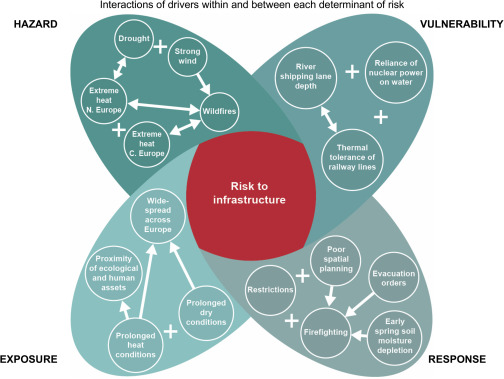
\includegraphics{figures/02_literature_review/simpson-risk-framework.jpg}
    \caption{A framework for decomposing risk into its parts: hazard, exposure,
    vulnerability, and response, using risk to infrastructure as an illustrative
    example. Reproduced from Simpson et al. (2021)
    \cite{simpson_framework_2021}.}
    \label{fig:risk-framework}
\end{figure}

\begin{figure}
    \centering
    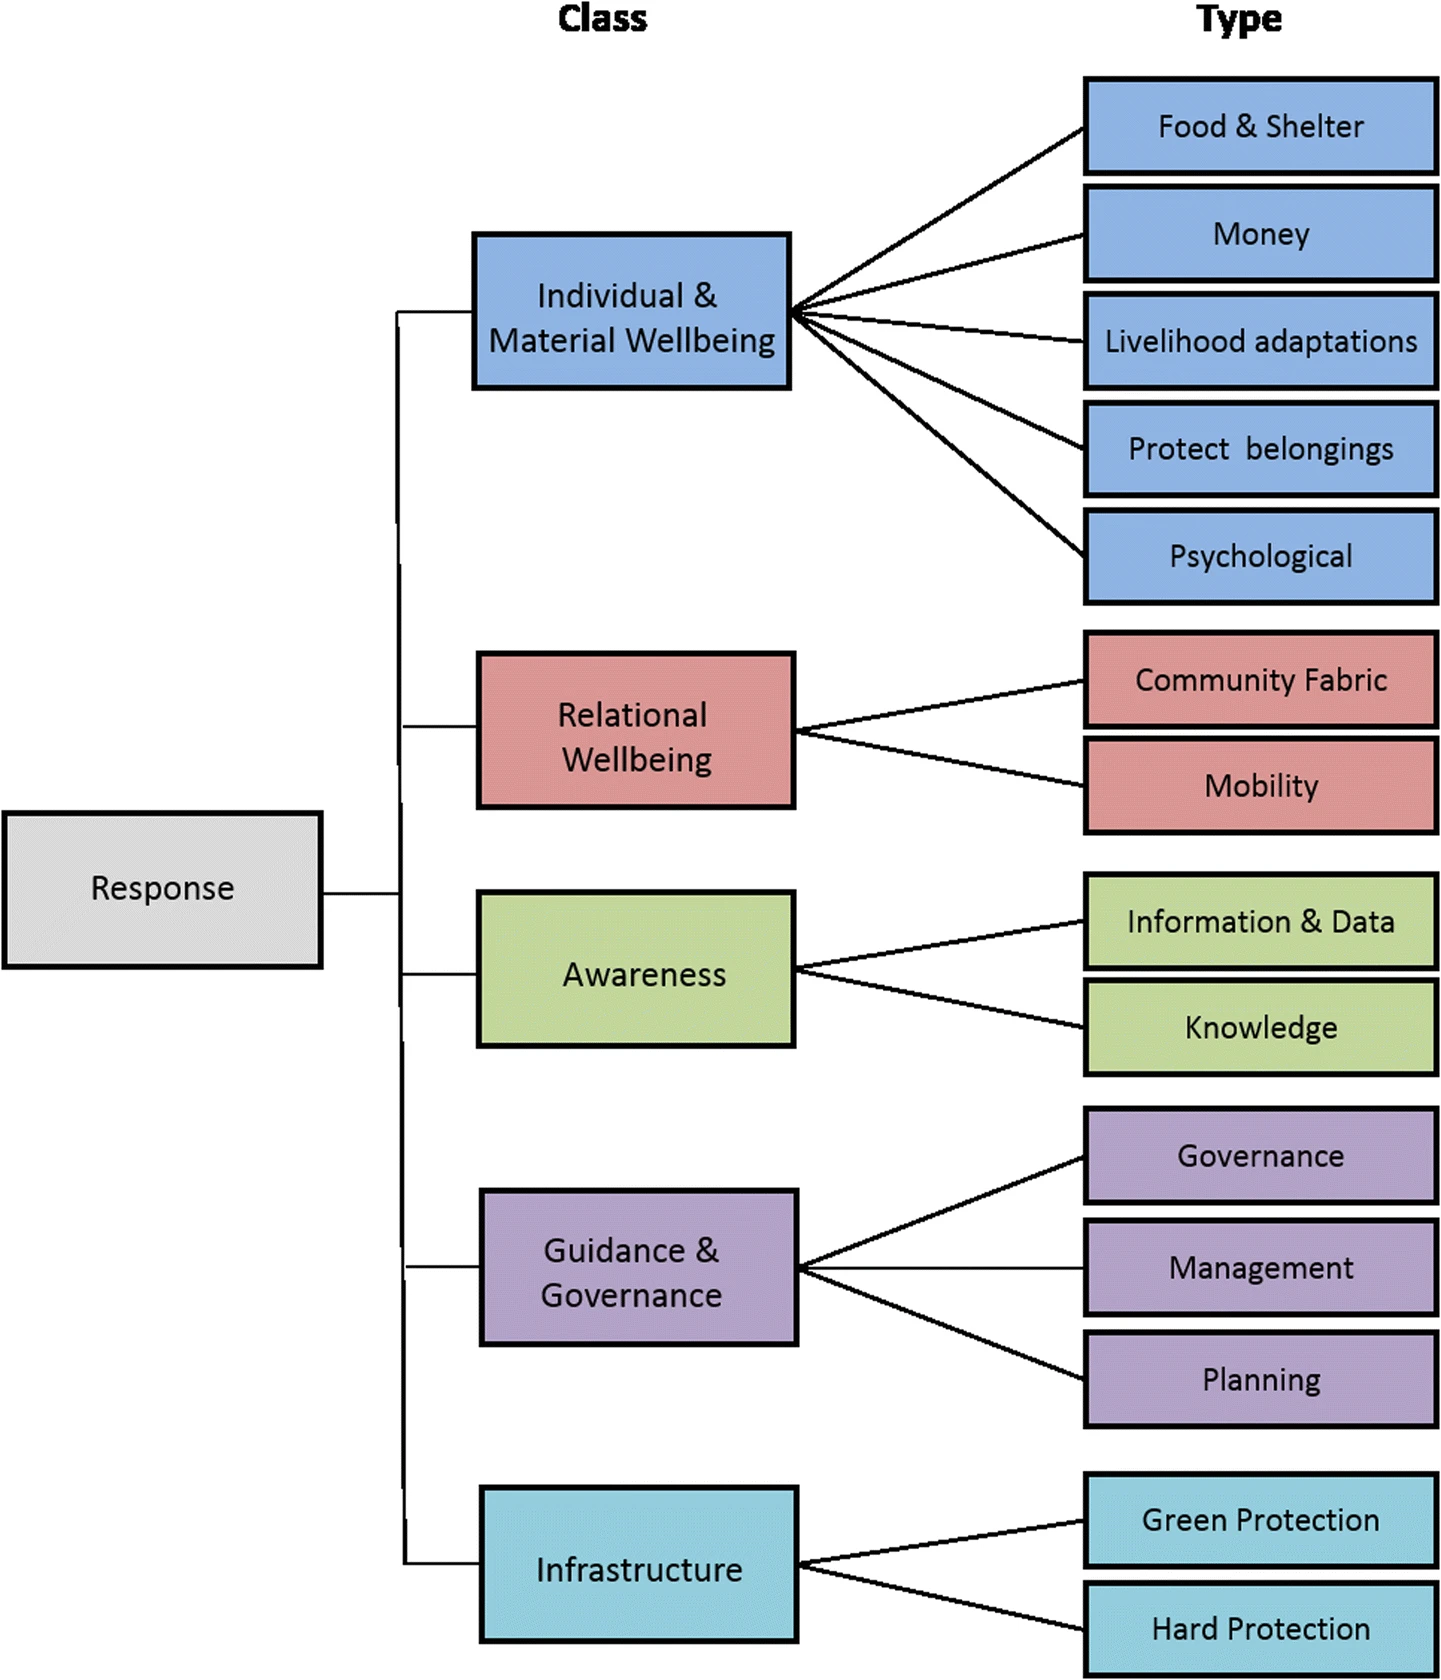
\includegraphics[width=\columnwidth]{figures/02_literature_review/risk-response.png}
    \caption{A categorization typology for various responses to climate risks.
    Reproduced from Paterson et al. (2019)
    \cite{paterson_community-based_2019}.}
    \label{fig:risk-response}
\end{figure}

% \noindent\hrulefill \item What are the responses to climate change? How
% successful have climate policies been at achieving climate goals (and
% ultimately achieving net zero carbon emissions)?

Based on the net-zero carbon emissions target set by the 2016 Paris Agreement,
myriad countries, states, and companies have set climate policies covering
two-thirds of the global economy \cite{hale_assessing_2022}. Reducing \ac{co2}
(or \ac{co2eq} in some cases) emissions is the primary focus for most of these
policies \cite{fawzy_strategies_2020, roelfsema_taking_2020,
hale_assessing_2022}, which include the following broad strategies
\cite{fawzy_strategies_2020}:
\begin{enumerate}
    \item Reducing \ac{ghg} emissions by transitioning from fossil-fueled to
    clean energy.
    \item Removing \ac{co2} from the atmosphere using \ac{ccs} and other
    sequestration techniques.
    \item Altering the Earth's energy balance by increasing its albedo and other
    geoengineering concepts.
\end{enumerate}
Despite this, only around five percent of these policies are consistent with the
\ac{un} ``Race to Zero'' campaign \cite{hale_assessing_2022}. Further, even the
full implementation of national climate policies leaves approximately  a 28
Gt\ac{co2eq} gap in \ac{ghg} emissions \cite{roelfsema_taking_2020} (with the
implicit goal of zero emissions). This gap and the fundamental assumptions about
carbon sequestration from the 2016 Paris Agreement suggest that the world is on
track to overshoot these emissions targets
\cite{roelfsema_taking_2020,taylor_managing_2021}. Carley et al. (2018)
developed a quantitative framework for assessing the vulnerabilities associated
with energy policies or responses \cite{carley_framework_2018}.

% \noindent\hrulefill \item What are the impacts of climate change?

Risk analysis is the first step to a more encompassing understanding of the
climate crisis. The literature on disproportionality further distinguishes
\textit{risks} and \textit{impacts} \cite{dorkenoo_critical_2022}. Consistent
with previous work, a risk is the aggregate of hazards, exposures,
vulnerabilities, and responses. Impacts, then, are the realizations of risk in
terms of loss and damages. This distinction is essential. Responses to
\textit{impacts} are always made \textit{ex post facto}. Differences in
vulnerability to a hazard, often arbitrated by socio-economic status, manifest
as differential impacts. Access to resources conditions an individual's or
community's ability to respond to the impacts of a hazard. Since losses from
impacts disproportionately affect those with the fewest resources, their
vulnerability to future hazards increases in a ``vicious cycle''
\cite{islam_climate_2017, dorkenoo_critical_2022}. In purely economic terms,
studies estimate the loss of ecosystem services from land use change associated
with climate change and other human activities at \$4 - \$20 trillion per year
(in 2011 \$US) globally, \cite{costanza_changes_2014} and the poorest third of
U.S. counties will experience financial damages between 2 and 20 percent of
their annual income \cite{hsiang_estimating_2017}. However, impacts also have
cultural and psychological dimensions \cite{dorkenoo_critical_2022} that cannot
be captured by accounting for ``externalities.''

% \noindent\hrulefill

% \item How are the damages of climate change distributed, and \textit{why} are
% they distributed this way?

Dorkenoo et al. \cite{dorkenoo_critical_2022} establish \textit{burdens},
injustices arising from social, political, or economic power imbalances, as a
third theme paramount for a holistic understanding of disproportionality.
Burdens influence all aspects of risk and affect access to resources which
condition impacts. Dorkenoo et al. wrote, ``[p]rocesses of marginalization and
exclusion influenced by power struggles [...] influence the distribution of
burdens and consequently responsibilities, in addition to the different
dimensions of climate risk (hazard, exposure, vulnerability [, response])''
\cite{dorkenoo_critical_2022}. Figure \ref{fig:risk-impact-burden} demonstrates
the mutually reinforcing relationships among risks, impacts, and burdens. A
particularly relevant example of burden is the persistence of energy burden,
where low-income households pay the highest percentage of their income on energy
bills relative to other income groups \cite{brown_high_2020,
cong_unveiling_2022}. Energy burden interferes with electricity access, thereby
increasing vulnerability to extreme heat events \cite{cong_unveiling_2022,
klinenberg_heat_2003}. The risk assessment literature and the energy system
modeling literature typically adopt an apolitical framing of vulnerabilities.
That is to say, these literature analyze their respective systems independent of
any sociopolitical context. However, inequities do not arise in a vacuum but
through processes of marginalization and exclusion
\cite{thomas_explaining_2019}. Often the distribution of burdens falls along
class, race, and gendered lines \cite{thomas_explaining_2019,mohai_which_2015}.
Research on siting patterns of polluting facilities indicates these projects
frequently developed in areas with people of color and low-income populations
\cite{mohai_which_2015}. Pollution from these facilities creates additional
burdens for nearby communities. The energy justice and environmental justice
literature offer insights to contrast this neutral framing and facilitate
normative questions about alternative distributions
\cite{dorkenoo_critical_2022, thomas_explaining_2019}.

\begin{figure}
    \centering
    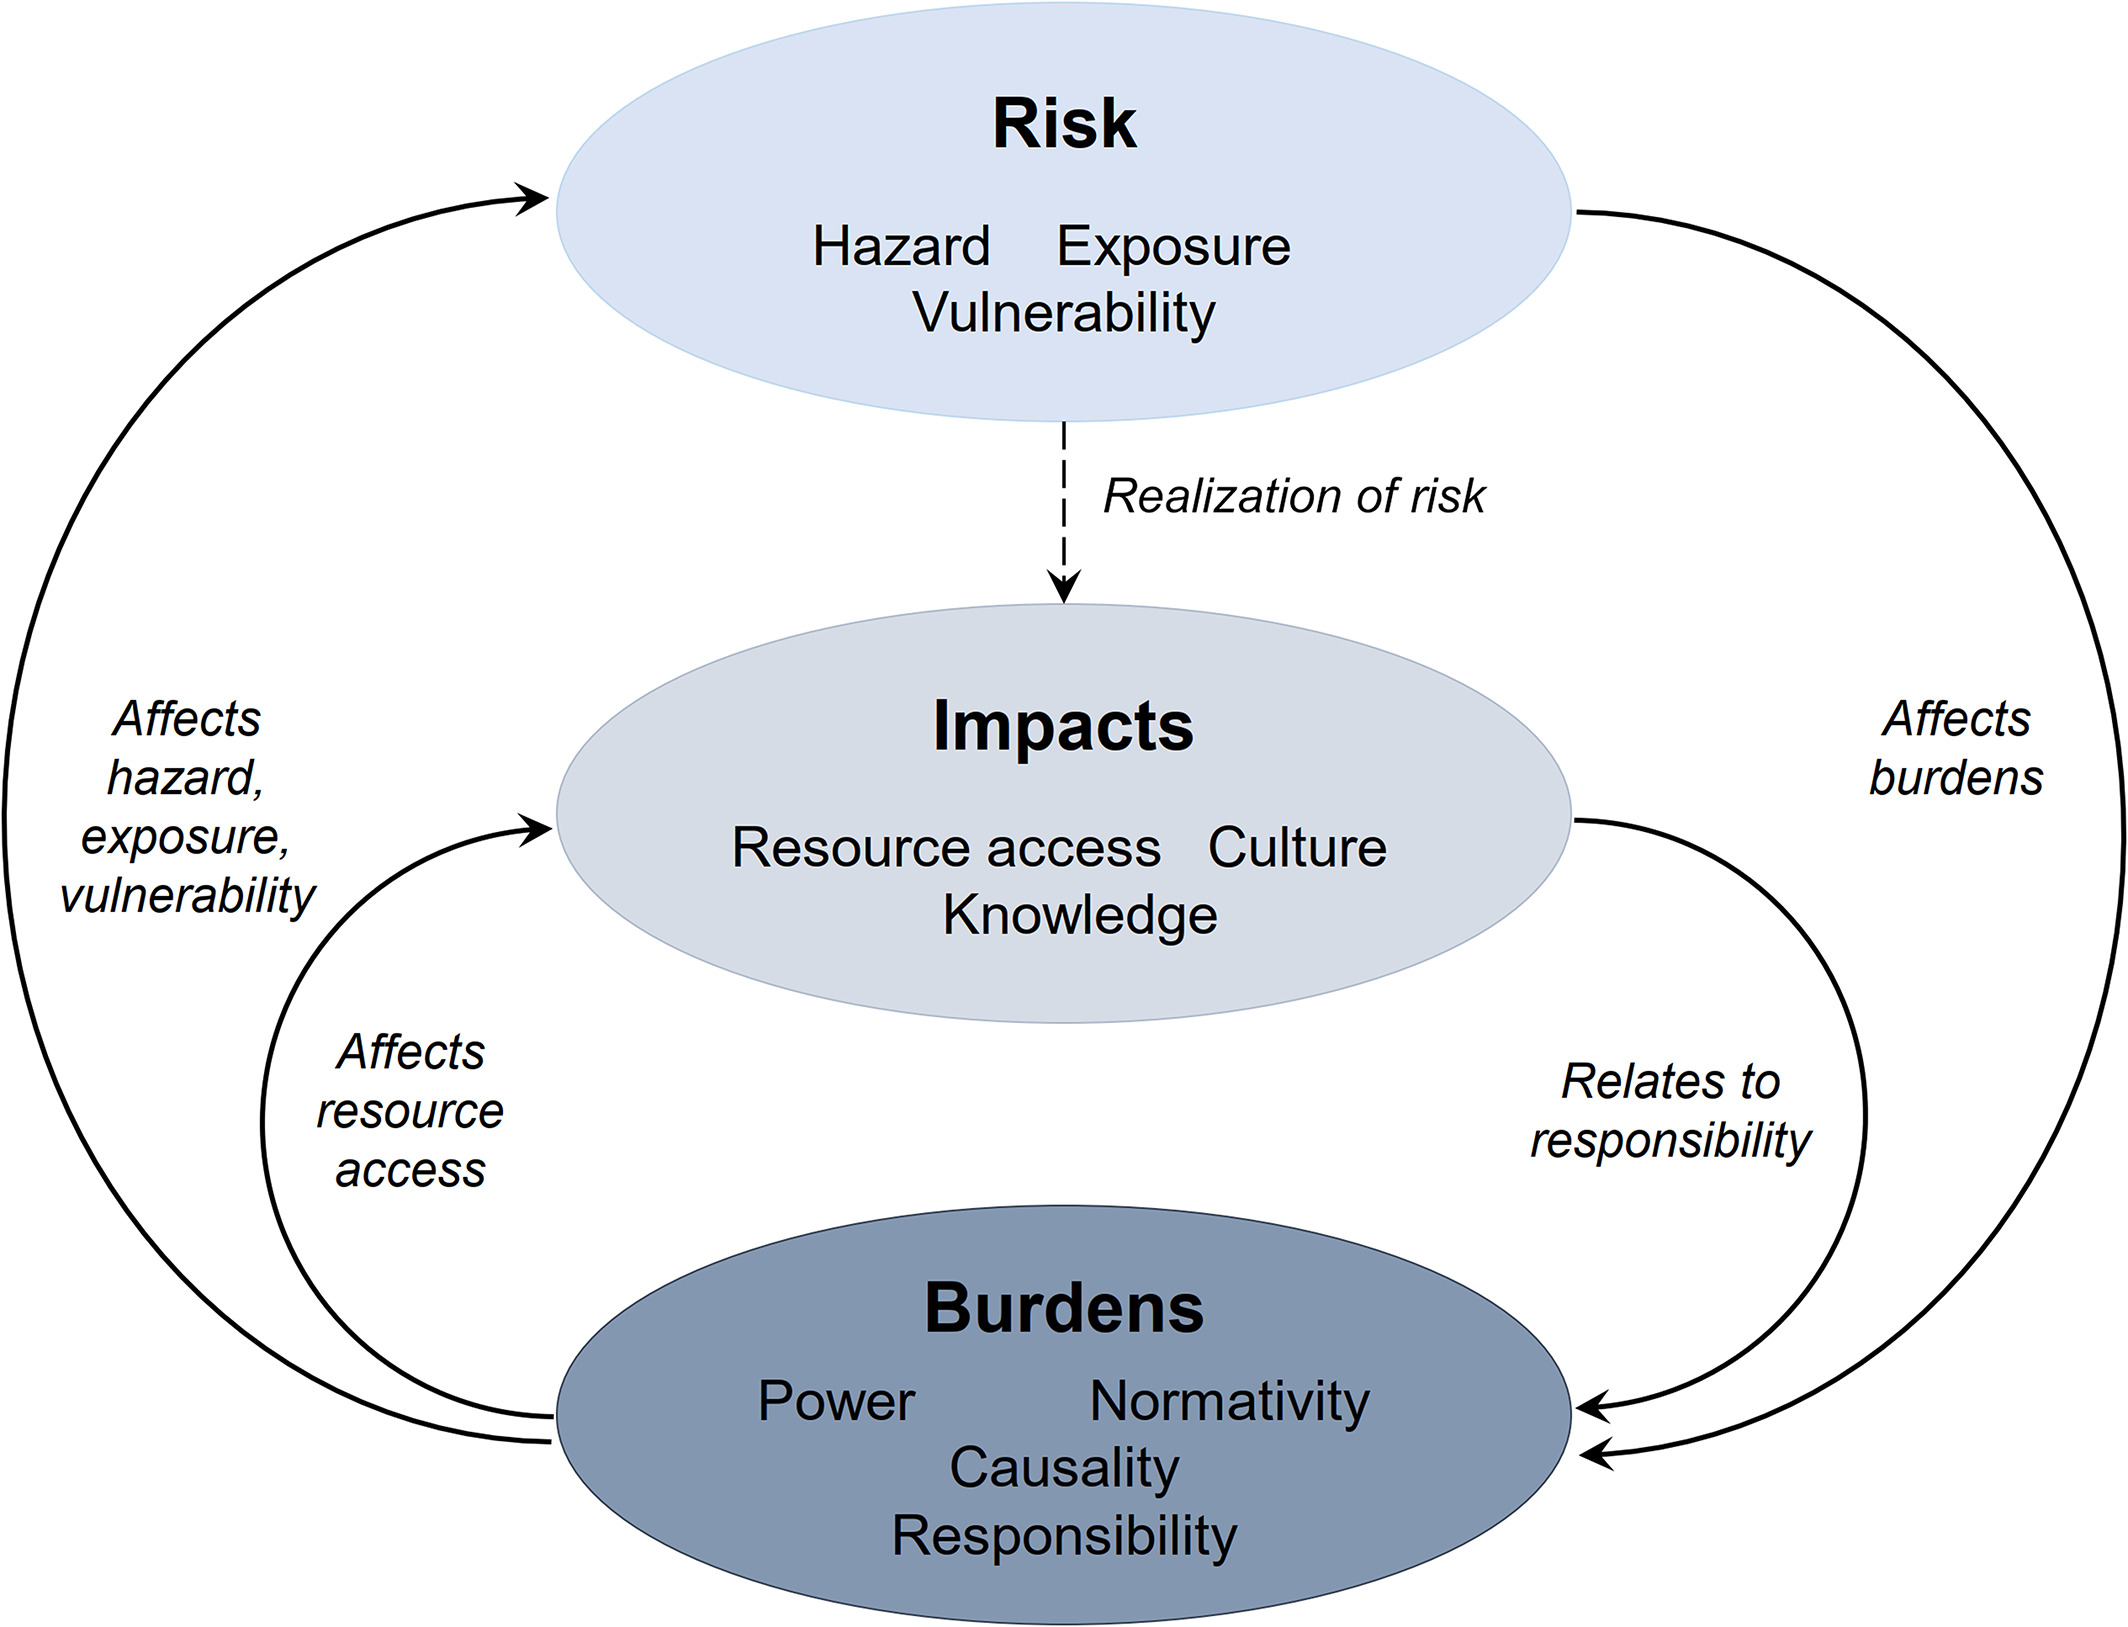
\includegraphics[width=\columnwidth]{figures/02_literature_review/dorkenoo-disproportionality.jpg}
    \caption{The relationships among risks, impacts, and burdens. Reproduced
    from Dorkenoo et al. (2022) \cite{dorkenoo_critical_2022}.}
    \label{fig:risk-impact-burden}
\end{figure}


% \noindent\hrulefill

% \textcolor{red}{Subsection: Climate and Energy Systems}
\section{Climate and Energy Systems}

Climate change is driven by the buildup of additional \acp{ghg} in our
atmosphere from human activities. \acp{ghg} are a significant byproduct of the
infrastructure that creates, delivers, and consumes energy (i.e., energy
infrastructure). The total decarbonization of the global economy will lead to
greater electricity demand, even when accounting for efficiency improvements
\cite{national_academies_of_sciences_engineering_and_medicine_accelerating_2021,
mai_electrification_2018}, decarbonizing our electricity production is one of
the most critical issues to resolving climate change. Therefore, producing
electricity with zero \acp{ghg} will initiate a cascade of deeper
decarbonization throughout the economy. However, this will require expanded
electrical infrastructure to accomodate new energy technologies. Since, energy
production contributes significantly to climate change, and new energy
infrastructure is required to reduce carbon emissions in other sectors (e.g.
heat and transportation), accelerating the adoption of clean energy technology
(i.e. technologies that do not release \acp{ghg} to the atmosphere) is essential
for achieving a stable climate \cite{roelfsema_taking_2020,
taylor_managing_2021}. The next section discusses the range of technical
solutions for accomplishing the goals established above.

% \textcolor{red}{Subsubsection: Technical solutions to energy decarbonization}
\subsection{Technical Solutions to Energy Decarbonization}
% \item What are the technical solutions for decarbonizing the electricity
% sector?

Many studies show that global and local economies can be supported by 100\%
\ac{vre}, such as wind, hydro, solar power, and storage \cite{jacobson_100_2015,
bussar_optimal_2014,brown_response_2018,dorotic_integration_2019,wallsgrove_emerging_2021,
cochran_la100_2021,cosic_100_2012,traber_economically_2021,bogdanov_full_2021,
bogdanov_north-east_2016,
esteban_100_2018,yue_least_2020,neumann_near-optimal_2021}. Yet some countries
that transition to majority \ac{vre} observe higher carbon emissions or a
slower-than-expected reduction due to greater dependence on natural gas brought
on by the relative unpredictability of natural energy sources
\cite{wagner_co2_2021}. Other studies demonstrate that firm baseload power, such
as nuclear power, is necessary for the deep decarbonization of our energy
systems
\cite{wagner_co2_2021,shaner_geophysical_2018,dotson_influence_2022,greene_enhancing_2019,kim_carbon_2021,
lehtveer_how_2015,vaillancourt_role_2008,
de_sisternes_value_2016,alzbutas_uncertainty_2012,brook_why_2014,
epiney_economic_2020,petti_future_2018, patrizio_socially_2020}. While some
countries are building new nuclear reactors, and the \ac{nrc} just licensed the
design of the first small modular reactor design from NuScale
\cite{office_of_nuclear_energy_science_and_technology_nrc_2023}, other places
are shutting down their operating nuclear plants \cite{johnson_new_2021}. 
% In the latter cases, places that shut down nuclear plants always saw a
% subsequent rise in carbon emissions due to greater dependence on natural gas.
% \textcolor{red}{Show plot of carbon emissions vs time for New York?}. 
Further, the only examples of highly decarbonized electrical grids are places
with a high penetration of hydro or nuclear power and the former is largely
exhausted in the United States \cite{lopez_us_2012}. Further, decarbonizing
electricity requires phasing out fossil-fueled power plants and a significant
expansion of clean electricity generators. Although many studies show the
\textit{feasibility} of a variety of energy mixes, the following is strongly
debated in the literature.
\begin{enumerate}
    \item Whether energy systems should be 100\% renewable or if nuclear power
    and \ac{ccs} should be included \cite{heard_burden_2017,
    brown_response_2018,elmallah_frontlining_2022, brook_why_2014}.
    \item What the role of distributed and decentralized energy sources in
    expanding our energy infrastructure should be
    \cite{pitt_assessing_2015,rinaldi_what_2022,parag_electricity_2016,wang_modeling_2020,
    morvaj_decarbonizing_2017,gilbert_can_2020,li_economic_2016,falke_multi-objective_2016}.
\end{enumerate}
The strength of the technical arguments on both sides of these discussions
combined with the distinct lack of sufficient policy agendas pursuing any of
them \cite{roelfsema_taking_2020,hale_assessing_2022}, suggests the existence of
poorly articulated trade-offs and that technical solutions cannot be assessed
from an engineering perspective, alone. Some researchers and policymakers
disagree on technical grounds, while others disagree on the basis of
institutional or systemic injustices. There are also differences in values.
Indeed, the cultural theory of risk argues that our social constructions, rather
than risks themselves, dictate what threats are recognized and their
corresponding liabilities and benefits \cite{mcneeley_cultural_2014,
van_de_graaff_understanding_2016}. Clean technologies like nuclear power and
renewables, such as solar or wind power, are not only different in how they
produce electricity but also in the values and paradigms they represent.
Sometimes, communication fails because the question being discussed is not
agreed upon either. Often, feasibility studies address the positive question,
``what is the least-cost pathway to the energy transition,'' while others
consider more normative questions, such as ``how should we proceed equitably?''\footnote{
    A \textit{positive} question is one that deals with factually
verifiable claims based on measurable data and are perceived as objective. For
example, asking ``what is the temperature outside'' is a positive question
because it asks what \textit{is} and can be answered by taking a measurement.
\textit{Normative} questions engage with ethics, judgement, and values. ``What
should I wear to go outside'' is a normative question because it asks what one
\textit{ought} to do \cite{hands_positive-normative_2012}.} Normative questions
are qualitative and, therefore, inherently challenging to answer and require the
application of ethics. Indeed there are many more normative questions than
positive ones. \textcolor{black}{Is perfect the enemy of good? How do we balance
stakeholder preferences, upstream and downstream effects, and the necessity to
respond quickly to climate change? Will this mix of influences lead to paralysis
or inaction?} Engineers typically do not possess the training nor the expertise
to answer these questions thoroughly. \textcolor{black}{Therefore, given climate
change's complex, interacting, and disproportionate nature, engineering alone is
ill-equipped to resolve the problem. Ideas from the environmental and energy
justice literature offer a social perspective for addressing the risks and
impacts of climate change hazards.} The next section introduces the concept of
energy justice and how this area of scholarship understands challenges related
to climate change and energy systems.


% \subsection{\textcolor{red}{If nuclear energy can solve climate change, where
are all the reactors?}}


% \begin{enumerate}
% \item What do proponents of nuclear energy say about nuclear power?
% \begin{itemize}
%     \item Nuclear engineers generally understand that discomfort and fear around
%     nuclear power come from fears about nuclear weapons and fears about
%     radiation. As such, they view these fears as irrational and placatable by
%     "educating" and ignorant public.
%     \item Some general benefits of nuclear energy (high energy density, low
%     material requirements, low carbon footprint, "safe," low land requirements,
%     reliable, "resilient").
%     \item Additionally, advocates for nuclear energy point to the sustainability
%     of nuclear energy due to its high energy density which in turn reduces the
%     amount of harmful externalities associated with its fuel cycle, relative to
%     other technologies.
%     \item Finally, the nuclear industry has a clear understanding of its fuel
%     cycle, the ways nuclear materials may be reused and/or disposed of, and the
%     measures needed to ensure its safety.
% \end{itemize}
% \item What are the technical objections to nuclear?
% \begin{itemize}
%     \item Nuclear accidents
%     \item Waste (high level waste is a tremendous issue.)
%     \item Ethical issues around mining (what historical harms have been done to
%     mining communities? What about sourcing uranium from places like Kazakhstan
%     (allied to Russia) and directly funding the invasion of Ukraine? What
%     reparations have been made to those harmed? How will future harms be
%     prevented?)
%     \item Nuclear weapons proliferation (discuss the relationship between
%     nuclear energy and nuclear power. Additionally, although nuclear power
%     doesn't necessarily lead to weapons programs, the need to keep careful track
%     of nuclear materials and prevent its release into the biosphere, malicious
%     or otherwise, presents a profound responsibility with some intergenerational
%     inequities).
%     \item Nuclear energy is expensive.
% \end{itemize}
% \item What are some non-technical critiques of nuclear power?
% \item Why are engineering solutions insufficient?
% \begin{itemize}
%     \item Case study on yucca mountain + sweden + finland
%     \item Are advanced reactors actually being designed in a way that
%     incorporates people's preferences. Perhaps preferences toward nuclear energy
%     are not so dependent on the probability of an accident, but on the trust
%     between reactor owners and host communities. Non-experts don't have the
%     expertise to assess the importance of neutron spectra, fuel form, or other
%     technical design parameters that are important for safety. Asserting a low
%     accident probability does not inspire trust. If the reactor is so safe, why
%     not put your money where your mouth is (so-to-speak) and engage in profit
%     sharing with the community? ``Communities are not the final arbiters of
%     safety, determining safety is the purview of the Nuclear Regulatory
%     Commission.''


%     \textcolor{red}{Should I include a question about the benefit of
%     profit-sharing in human-subjects interviews? What are their concerns with
%     energy? Are they focused only on the production of energy or also the
%     lifecycle (extraction + disposal) as well?}
% \end{itemize}
% \end{enumerate}


%What do proponents of nuclear energy say about nuclear power?

In spite of its complicated history, nuclear energy has a variety of unique
benefits that researchers and advocates cite to support its continued and
expanded use. First, uranium has an enormous energy density. This fact has a
number of important consequences that favor the use of nuclear energy, such as
low land use \cite{lovering_land-use_2022,van_zalk_spatial_2018}, high \ac{eroi}
\cite{weisbach_energy_2013,murphy_energy_2022}, and a low mass and volume of
waste byproducts relative to other sources
\cite{liu_wind_2017,chowdhury_overview_2020,holdsworth_spent_2023,taebi_recycle_2008}.
Second, due to the nature of nuclear fission, nuclear power plants emit zero
carbon emissions, making them among the ``cleanest'' sources of energy along
with solar panels and wind turbines
\cite{nicholson_life_2021,intergovernmental_panel_on_climate_change_climate_2021,
brook_why_2014,van_de_graaff_understanding_2016}. Third, nuclear reactors
produce reliable baseload electricity and have the highest capacity factor of
any energy generating technology
\cite{brook_why_2014,van_de_graaff_understanding_2016}. Advocates for nuclear
energy also argue that nuclear energy is among the ``safest'' energy sources,
measured in deaths per unit energy produced
\cite{brook_why_2014,van_de_graaff_understanding_2016,sovacool_balancing_2016}.


%What are the technical objections to nuclear?
Although there are genuine benefits to producing electricity with nuclear
energy, concerns over its use persist. Nuclear engineers generally understand
that discomfort and fear around nuclear power come from fears about nuclear
weapons, nuclear plant accidents, and nuclear waste \cite{roeser_nuclear_2011}.
Each of these concerns are reflected in a different part of the nuclear fuel cycle,
shown in Figure \ref{fig:nuclear-fuel-cycle}.

\begin{figure}[ht]
    \centering
    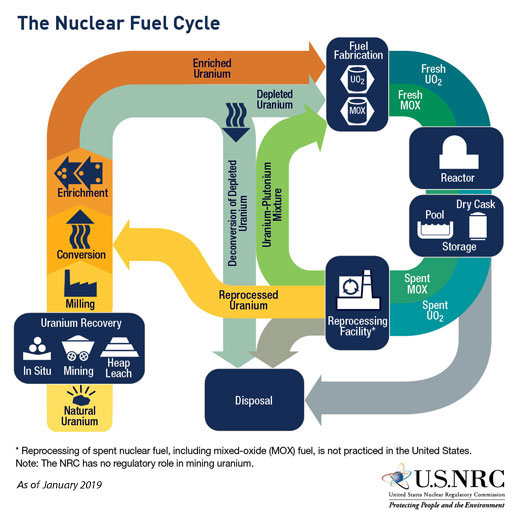
\includegraphics[width=0.5\columnwidth]{figures/nuclear-fuel-cycle-02.jpeg}
    \caption{Stages of the nuclear fuel cycle. Reproduced from \cite{nuclear_regulatory_commission_stages_2020}}
    \label{fig:nuclear-fuel-cycle}
\end{figure}

\noindent
Engineers typically adopt a ``hierarchical'' attitude, as described by cultural
theory of risk \cite{van_de_graaff_understanding_2016,mcneeley_cultural_2014},
and thus perceive these fears as irrational and placatable by ``educating'' an
ignorant public; consistent with the ``deficit model'' of science communication
\cite{simis_lure_2016,patenaude_topical_2022}. \textcolor{red}{It is incumbent
on nuclear engineers and advocates to adequately communicate the risks
associated with nuclear energy and not dismiss concerns due to a lack of
technical rigor.} Although \ac{snf} (commonly ``nuclear waste'') does not
present an immediate risk for radiological release, the details around managing \ac{snf} require
thoughtful consideration. Choosing between an open or a closed nuclear fuel
cycle implies different ethical foundations. Specifically, the tradeoff between
long- and short-term risks that must be carefully weighed
\cite{taebi_recycle_2008}. Further, even though civilian nuclear energy has not
led to the proliferation of nuclear weapons
\cite{herzog_nuclear_2020,miller_why_2017}, the need to keep careful track of
nuclear materials and prevent its release into the biosphere, malicious or
otherwise, presents a profound responsibility with some intergenerational
inequities. Finally, there are elements of the nuclear fuel cycle that 
are frequently ignored. In particular, mining and fuel fabrication are 
often overlooked by advocates for nuclear energy, even though mismanagement in these parts of
the nuclear fuel cycle have led to significant environmental disasters, such as the 
accident in Church Rock, New Mexico \cite{moore-nall_legacy_2015,rojavin_civilian_2011}. 

In addition to these ethical and technical issues, some have argued that, due to the
risks discussed above, nuclear energy requires centralized and authoritarian decision-making
structures and is therefore anathema to inclusive and democratic
values \cite{van_de_graaff_understanding_2016, winner_artifacts_1980}. However, conversations
within the nuclear spaces have reopened this question about the implicit ``politics'' of nuclear
energy, spurred on by the development of \acp{smr} \cite{lovering_social_2021}.

Distinct from conversations surrounding the ethics and risks of using nuclear
energy, many nuclear energy skeptics insist that nuclear power is too expensive
to support decarbonization goals. While it is true that nuclear power plants
have significant capital costs \cite{nrel_2020_2020} which have grown in many
countries due to additional regulations and safety requirements (i.e.,
``negative learning'') \cite{lovering_historical_2016}, it remains unclear
whether these costs uniquely translate to burden on electricity consumers.
Especially given nuclear energy's role as a ``price-taker'' in electricity
markets \cite{murphy_impacts_2019} and evidence for nuclear's stabilizing effect
on electricity prices \cite{dotson_influence_2022,de_sisternes_value_2016}.

 
% \subsection{\textcolor{red}{If renewable energy can solve climate change, why
build anything else?}}

\begin{enumerate}
    \item What do proponents of renewable energy say about solar and wind?
    \begin{itemize}
        \item By virtue of being renewable, the ``fuel'' source is practically
        infinite. Solar energy will never run out on the timescale of human
        civilization, and wind energy (as a product of wind energy plus the
        Earth's rotation) will similarly never run out.
        \item Since renewable energy, specifically solar and wind, lend
        themselves more naturally to distribution, they are more democratic
        sources of energy (cite).
    \end{itemize}
    \item What are the technical objections to fully renewable energy grids?
    \begin{itemize}
        \item Wind and solar are variable and intermittent energy sources.
        \item Renewable energy sources (including non-intermittent sources like
        hydroelectric dams and biomass) have a much lower \ac{eroi} than fossil
        fuel sources \cite{hall_eroi_2014,weisbach_energy_2013}. However, recent
        harmonization studies belie this assertion by demonstrating that
        renewable sources have similar, if not greater, \ac{eroi} than coal or
        natural gas \cite{murphy_energy_2022}.
        \item Although the ``fuel'' for solar and wind resources is infinite,
        the materials required to extract energy from these sources is finite.
        \item In contrast with the nuclear energy, the renewable energy industry
        does not have a strong notion of the lifecycle of their technology.
        There are no plans to safely store or recycle solar panels and wind
        turbines at end-of-life.
    \end{itemize}
    \item What are some non-technical objectives to renewable energy?
    \begin{itemize}
        \item Democracy and inclusivity are not required features of renewable
        energy sources \cite{bell_toward_2020,winner_artifacts_1980}. Although
        renewables have the potential to be highly decentralized, this is not a
        requirement of their use. Many deployment schemes for solar and wind
        farms involve creating highly centralized ``farms'' that are owned and
        operated by a single corporate entity, thereby recreating the same power
        structures that currently exist and thus perpetuating inequities.
    \end{itemize}
    \item What drives the opposition for renewable energy projects (specifically
    wind and solar)?
    \begin{itemize}
        \item Due to the sprawling nature of energy sources like solar and wind,
        these projects are frequently subject to public opposition in proposed
        areas.
        \item The \ac{nimby} movement, or \acs{nimbyism}, is frequently cited as
        the cause of opposition (cite). \ac{nimbyism} describes people that do
        not support the execution of a specific project (energy-related or
        otherwise) due to the project's proximity to a certain location
        (typically residences), but would otherwise support a project if it were
        further away. Despite the popular understanding of \ac{nimbyism}'s role
        in delaying energy projects, the most comprehensive empirical research
        on \ac{nimbyism} demonstrated that \ac{nimby} attitudes do not drive
        public opposition \cite{konisky_proximity_2021}. 
    \end{itemize}
\end{enumerate}

% What do proponents of renewable energy say about solar and wind?

Renewable energy sources, particularly solar and wind energy, are appealing
alternatives to fossil fuel sources. Solar and wind energy have fewer
geographical constraints, compared to hydroelectric and geothermal power
\cite{lopez_us_2012}. With respect to nuclear energy, solar and wind are
similarly safe on a per-unit-energy basis and produce comparable lifecycle
carbon emissions
\cite{united_nations_economic_commission_for_europe_carbon_2022,sovacool_balancing_2016,
intergovernmental_panel_on_climate_change_climate_2014}. Contrary to popular
belief, solar and wind resources can have \ac{eroi} comparable to coal-fired
power plants \cite{murphy_energy_2022}.
% \subsection{\textcolor{red}{Current procedures}}


\textcolor{red}{In this section I want to cover the current issues related to siting 
energy projects and how they are executed. This should relate issues identified in the case studies
for siting a nuclear waste repository (as well as the successes!) and the challenges of siting renewable
energy projects. Once I have made this connection, I can summarize the case study on the Dakota Access Pipeline
done by McKenzie Johnson \cite{johnson_dakota_2021}. I can also refer to the process for obtaining a nuclear
reactor license.
Finally, it may be useful to identify a ``successful'' siting process? Such as the siting of a transmission line
in Ireland \cite{devine-wright_understanding_2020}.
This section also serves as a great segu\'{e} into discussions of energy justice. Since engineers are not 
typically equipped to do the kind of public engagement required to advance energy goals.}
% \noindent\hrulefill \textcolor{red}{Subsubsection: Energy justice and the
% Boundaries of Energy Systems.}
\section{Energy Justice}
\label{section:energy-justice}
% \item What is energy justice?


Energy justice is a conceptual and analytical tool regarding the ethical or
normative dimensions of energy systems and addresses the systemic causes of
burdens, and inequities \cite{sovacool_energy_2015}.
% \begin{enumerate} \item What is justice?
    There are many conceptions of justice; however, the most popular framework
    for understanding justice is a three-faceted approach originating from David
    Schlosberg: distributive, recognition, and procedural justice
    \cite{schlosberg_2_2007}.
    % \item What is distributive justice? 
% \noindent\hrulefill
    Distributive justice relates to the fair distribution of resources,
    burdens, and responsibilities. Studies on distributive justice seek to
    address the normative question: how should a just society distribute the
    benefits it produces and \textit{the burdens required to maintain it}
    \cite{brighouse_justice_2004}. Additionally, distributive justice
    considers \textit{how} poor distributions are created
    \cite{schlosberg_2_2007}.
% \noindent\hrulefill
    % \item What is procedural justice?
    Procedural (in)justice is defined as the presence of (un)fair and
    (in)equitable institutional processes of the state \cite{schlosberg_2_2007}.
    In other words, how decisions of societal import are made and who is
    involved in those decisions. Sovacool and Dworkin (2015) outline four
    elements of procedural justice: transparency, meaningful participation,
    impartiality, and avenues for redress \cite{sovacool_energy_2015}.    
% \noindent\hrulefill
    % \item What is recognition justice?
Justice of recognition is the most vague of the three tenets of justice and is
    frequently reduced to a component of either distributive or procedural
    justice \cite{schlosberg_2_2007, van_uffelen_revisiting_2022}. A common
    argument for this consolidation is that recognition is a precondition for
    achieving distributive justice or that achieving procedural justice
    necessarily includes recognition \cite{schlosberg_2_2007}. However,
    recognition is unique from distributive and procedural justices because it
    is concerned with a different family of injustice, namely,
    \textit{misrecognition} \cite{van_uffelen_revisiting_2022}. van Uffelen
    (2022) suggests a nuanced definition of recognition justice as ``the
    adequate recognition of all actors through love, law, and the status order''
    \cite{van_uffelen_revisiting_2022}.
% \end{enumerate} \noindent\hrulefill
Sovacool and Dworkin (2015) offer a framework for assessing energy policies from
a justice perspective. Table \ref{tab:justice-frameworks} map the relationships
between justice-as-a-decision-making-tool from Sovacool \& Dworkin, Paterson's
hazard response characterization, and Schlosberg's triumvirate of justice. 

\begin{table}[h]
    \centering
    \caption{Different ways to operationalize justice concepts.}
    \input{tables/justice-approaches.tex}
    \label{tab:justice-frameworks}
\end{table}

Although Sovacool \& Dworkin do not explicitly discuss recognition justice, it
is a unique aspect of justice that can still be useful for contextualizing their
recommendations. For example, due to the psychological pressures introduced by a
lack of access to energy, either due to infrastructure or cost, interrupts
relational well-being and is an injustice \cite{van_uffelen_revisiting_2022}.
Further, (un)sustainable policies may be considered a misrecognition of the
humanity of future generations. Next, I examine the specific ways the social
science literature understands how energy systems and their infrastructure
(artifacts) contribute to the distribution of burdens.

% \noindent\hrulefill \item What is an energy system?
\subsection{Boundaries of Energy Systems}
\label{section:energy-system-boundaries}
Previous work defined energy systems in purely technical terms as spatially,
temporally, and topologically complex machines that coordinate the supply and
demand of energy, especially electricity \cite{dotson_influence_2022}. However,
this definition neglects the ways energy systems may be used to construct and
maintain power relations that contribute to inequitable distributions of
burdens. Energy access is necessary to support complex modern economies and
therefore possesses political power \cite{jones_building_2013,
bridge_energy_2018}. The literature on the political economy of energy
infrastructure locates this political influence in five distinct ways
\cite{bridge_energy_2018}. First, energy infrastructure affects competition and
collaboration among nation-states in the geo-political sphere. The current
situation in Ukraine makes this especially salient
\cite{figueiredo_impacts_2022}. 

The second subset of the literature focuses on the process of energy
infrastructure development and how these processes create social inequities. For
example, energy policies that subsidize residential solar panels have not led to
more equitable adoption of solar energy, with greater adoption in areas with
higher income, among other social indicators \cite{reames_distributive_2020}.
Other popular arguments in favor of renewable energy assert that these energy
sources are necessarily more egalitarian because the Sun and the wind cannot be
(or have not yet been) privatized. Another is the urgency of climate change.
Although these arguments have merit, they ignore or minimize the potential
environmental and social consequences of energy planning that does not consider
energy justice \cite{jones_building_2013}. Large-scale energy projects in the
Global South have already led to the dispossession of nearby indigenous
communities and other key actors \cite{yenneti_spatial_2016,
barragan-contreras_procedural_2022}.

Third, the development of energy infrastructure is not simply conducted via
policy measures, but also in the manner governments activate the public
imagination in favor of these policies
\cite{bridge_energy_2018,jasanoff_containing_2009}. Jasanoff and Kim (2009)
articulate this concept as `socio-technical imaginaries,' which are
simultaneously descriptive and prescriptive of possible energy futures
established by governments in the national zeitgeist
\cite{jasanoff_containing_2009}. This concept is demonstrated by the discourse
surrounding nuclear energy in the United States and South Korea
\cite{jasanoff_containing_2009} as well as in Japan
\cite{valentine_energy_2019}. Governments can employ `grand narratives' related
to national security, climate change, or modernization to enhance public support
while minimizing genuine participation \cite{bridge_energy_2018}.

Fourth, the political power of energy infrastructure can be traced further to
the cultural values and policy choices embedded in the design and operation of
seemingly technical systems \cite{bridge_energy_2018}. In other words, the
design and implementation of energy infrastructure may be used as a vehicle for
apparently unrelated agendas, a form of ``policy-making by other means''
\cite{bridge_energy_2018, clausewitz_chapter_1918}. Edwards and Hecht (2010)
refer to the co-constitution of technological and political order as
`\textit{technopolitics},' demonstrating the tangible material and political
outcomes of technological systems \cite{edwards_history_2010}.

Finally, energy systems and their infrastructure possess a unifying quality
through which new political identities may evolve \cite{bridge_energy_2018}.

From these various perspectives, we can observe that confining an energy system
to its technical characteristics is woefully incomplete. I propose that an
energy system is a spatially, temporally, and topologically complex machine that
coordinates the supply and demand of energy and resources and acts as an
important mediator of burdens that influence risks (such as risks from climate
change). This thesis takes the important step of analyzing energy system
planning and policy with this expanded definition. The next section reviews
current attempts to model energy systems and identifies gaps in conventional
methods.

% \textcolor{red}{Climate change \textit{is} a complex issue with multiple
% interacting and interwoven layers. However, it can and must be understood
% holistically instead of stripping it of its complexity and exclusively
% relegating solutions to the realms of economics and engineering. This
% over-simplification is done out of a misplaced sense of pragmatism and either
% an inability or unwillingness to completely apprehend the problem.}

% \noindent\hrulefill \item What are the obstacles to building more clean energy
% infrastructure? What is preventing the transition to a ``qualitatively new
% type of [environmental] society'' \cite{bluhdorn_legitimation_2020}?

% \textcolor{red}{This is where you can introduce different schools of thought
% about transitions.}

% \textcolor{blue}{Interesting that you chose to frame public acceptance as an
% ``obstacle'' rather than a source of greater accountability and
% participation.} \begin{enumerate} \item Legitimation crisis of democracy
% \cite{bluhdorn_legitimation_2020}. \item Social acceptance literature
% \end{enumerate}

% \end{enumerate}

% \section{Calls for a Just-Transition}

% Att


\section{Modeling Energy Systems}
\label{section:esoms}

Energy system optimization models (ESOMs)\acused{esom} have broad utility,
including forecasting future quantities, generating insight for policy
development, or energy system planning for scheduling and acquisition
\cite{decarolis_using_2011, yue_review_2018}. However, analyses using currently
available \acp{esom} seldom consider the role of energy systems in creating and
maintaining inequitable distributions of burdens. \acp{esom} vary significantly
by the energy sectors they choose to model, the degree of physical detail,
uncertainty quanitification, and forecasting capabilities. Table \ref{tab:esoms}
summarizes the capabilities for a comprehensive list of energy system analysis
tools. These tools are approximately sorted by mathematical formulation, e.g.
explicit optimization or simulation. The ``\ac{milp}'' column indicates whether
the framework uses a linear-programming approach to optimize an objective
function. The ``objective'' column specifies the nature of the objective
function if one exists. ``Cost'' objectives minimize total or annual energy
costs, while ``welfare'' maximizes social welfare. Some entries have more than
one objective listed. This means users may choose which objective to optimize.
None of the tools in Table \ref{tab:esoms} are designed to handle simultaneous
optimization (i.e., \ac{moo}). For those modeling frameworks that have an
``objective'' in Table \ref{tab:esoms}, virtually all of them optimize system
costs. EnergyScope is the only exception to this, which allows users to optimize
\ac{ghg} emissions \cite{limpens_energyscope_2019}. \textcolor{black}{The
``uncertainty'' column indicates a feature to algorithmically generate model
runs for testing either parametric or structural uncertainties.
\textcolor{black}{For example, EnergyScope is \textit{suitable} for uncertainty
analysis (i.e., many runs are computationally tractable) but does not have any
built-in capabilities \cite{limpens_energyscope_2019}.} Some tools, such as NEMS
\cite{nalley_national_2019}, incorporate uncertainty into their calculations via
learning curves. However, these learning curves require assumptions about
learning factors and technological ``optimism'' --  which are themselves
uncertain \cite{nalley_national_2019}.} Table \ref{tab:esoms} also indicates
whether the tool is a ``public code.'' This simply means users can download and
inspect the source code. Other considerations for openness, such as licensing
and development, vary among the listed frameworks. \textcolor{black}{The other
columns simply indicate the existence of particular features rather than the
relative maturity or sophistication of each feature.} 

Frameworks, such as MEDEAS \cite{capellan-perez_medeas_2020}, and MultiMod
\cite{huppmann_market_2014}, are general equilibrium models which embed energy
systems within the macro-economy and facilitate the modeling of strategic
behavior. The latter formulates a non-linear problem with the Karush-Kuhn-Tucker
optimality condition \cite{huppmann_market_2014}, as opposed to more traditional
linear programming methods. Models of this type are helpful for analyzing the
economy-wide influence of policies but lack sufficient operational detail to be
prescriptive for energy system planning.

\textcolor{black}{Agent-based models are useful for modeling the market
behaviors of different actors, such as firms (which produce power), transmission
operators, and consumers. The latter category is typically aggregated for
tractability. Modeled behaviors include technology preferences
\cite{anwar_modeling_2022, zade_quantifying_2020}, risk aversion
\cite{anwar_modeling_2022}, financial characteristics \cite{anwar_modeling_2022,
nitsch_economic_2021}, and information asymmetry among agents
\cite{anwar_modeling_2022, nitsch_economic_2021}. Due to agent heterogeneity,
agent-based models are considered useful for capturing social phenomena
\cite{yue_review_2018,fattahi_systemic_2020}.}

A further set of tools focus on simulating power flow and demand fluctuations.
\textcolor{black}{CAPOW \cite{su_open_2020} generates synthetic data with
statistical methods to explore uncertainties in energy dispatch and extreme
demand events, but does not include any investment optimization based on these
uncertainties.} \textcolor{black}{CESAR-P, SAM, Demod, and DESSTinEE focus on
modeling demand profiles
\cite{leoniefierz_hues-platformcesar-p-core_2021,bosmann_shape_2015,barsanti_socio-technical_2021}.
CESAR-P models individual building demand for energy based on the physical
parameters of the building. However, it has no dispatch or investment
optimization capabilities.} Other tools such as Pandapower, GridCal, and SciGRID
power model the infrastructure aspects of electricity systems -- transmission
and distribution -- rather than the optimal dispatch of electricity producers
\cite{thurner_pandapower_2018, vera_gridcal_2022, matke_structure_2017}.

There is an overwhelming number of models with varying levels sophistication and
capabilities. However, the inability to optimize any objective besides cost
presents a significant gap in the existing space of energy modeling tools.
Further, since none of these tools allow for multiple objectives, true trade off
analysis is rendered impossible.



\begin{table}
    \centering
    \caption{Summary of \ac{esom} frameworks.}
    \label{tab:esoms}
    \resizebox*{\textwidth}{0.95\textheight}{\input{tables/esom_database.tex}}
\end{table}
\FloatBarrier

% \begin{itemize} \item METIS has the following motivation
%     \cite{sakellaris_metis_2018} \begin{enumerate} \item Close the gap between
%     modellers and policy-makers, enabling policy-makers to become modellers.
%     \item reconciles user-friendliness with powerful capabilities \item
%     modularity \item \textcolor{red}{METIS does not support multi-objective
%     optimization!}    
%     \end{enumerate} \item energyRt has similar motivations
%     \cite{lugovoy_energyrt_2022}. \begin{enumerate} \item enhance
%     reproducibility \item reduce the learning curve \item minimize model
%     development time \end{enumerate} \item GENESYS cannot \sout{can} do
%     multi-objective optimization \cite{bussar_optimal_2014}. It uses a logical
%     flow to model dispatch behavior for a genetic algorithm! \begin{enumerate}
%     \item One drawback of the "hierarchical system management" method (i.e. a
%     logical flow chart) is the difficulty of modeling ramping rates... (test
%     this). \end{enumerate} \end{itemize}

\subsection{Economic Dispatch and Social Welfare}
\Ac{lp} or \ac{milp} are the dominant optimization approaches among the
frameworks in Table \ref{tab:esoms}. Economic dispatch models optimize the power
output of \textit{dispatchable} generators in a model system
\cite{de_queiroz_repurposing_2019, neumann_near-optimal_2021}. They all share
the same fundamental formulation.
\begin{align}
    \intertext{Minimize}
    \label{eqn:generic_objective}
    &F(x) = \sum_i C_i x_i\\
    % &F(x) = \sum_t^T\left[\sum_i^{N_g}{C_i^g x_i} - \sum_j^{N_d}{C_j^d x_j}\right],\\
    \intertext{subject to,}
    % &\sum_i{x_i} - \sum_j{x_j} = 0\\
    &g(x, p) \leq 0.\nonumber\\
    &x \in \vec{X}\nonumber\\
    \intertext{where}
    &\vec{X} \text{ is the set of decision variables,}\nonumber\\
    & C_i \text{ is the \textit{i-th} cost,}\nonumber\\
    & g \text{ is some linear inequality constraint,}\nonumber\\
    & p \text{ is some arbitrary parameter.}\nonumber
\end{align}
The exact formulation of Equation \ref{eqn:generic_objective} may vary slightly
across models, but the objective for most economic dispatch models is to
minimize total cost. The near universality of a cost-based objective function
comes from the concept of \textit{social welfare maximization}. This concept is
illustrated in Figure \ref{fig:social-max}.

\begin{figure}[H]
  \centering
  \resizebox{\columnwidth}{!}{\input{figures/02_literature_review/social_max.pgf}}
  \caption{Demonstration of ``social welfare maximization.'' Plot a) shows the
  total surplus when the price is at equilibrium. Plot b) shows the total
  surplus when the price is artificially depressed.}
  \label{fig:social-max}
\end{figure}

In microeconomics, social welfare is identical to the sum of consumer and
producer surplus. Therefore social welfare is maximized when the sum of these
two quantities is maximized. Figure \ref{fig:social-max} shows this case on the
left panel. However, suppose an economic policy capped the price of some product
at a price lower than the equilibrium price. In that case, the consumer surplus
expands, and the producer surplus contracts, as shown in the right panel of
Figure \ref{fig:social-max}. Nobody receives the ``lost surplus'' because
suppliers do not produce more despite unmet demand for the product because the
price is capped. Typically, modeling tools consolidate the demand curve to a
single value. \textcolor{black}{In this case, social welfare maximization is
approximated by minimizing the total cost of energy
\cite{richstein_cross-border_2014}}. This simplification is valid because demand
for energy is highly inelastic \cite{heuberger_power_2017, eia_price_2021,
labandeira_meta-analysis_2017, csereklyei_price_2020}. Figure
\ref{fig:inelastic} shows the impact of highly inelastic demand.

\begin{figure}[H]
  \centering
  \resizebox{\columnwidth}{!}{\input{figures/02_literature_review/elasticity.pgf}}
  \caption{Demonstration of ``price elasticity.'' Plot a) shows a typical supply-demand curve where changes in price lead to proportional changes in demand. Plot b) shows an inelastic demand where consumption does not change proportionally with price.}
  \label{fig:inelastic}
\end{figure}

For an elastic good supply and demand are in proportion with each other. An
increase in the supply leads to a proportional increase in demand via a reduced
price, eventually returning to an equilibrium price (shown in Figure
\ref{fig:inelastic}a). However, as Figure \ref{fig:inelastic}b demonstrates, an
inelastic demand does not respond proportionally to changes in price, such that
consumers become ``price- takers,'' paying the price set by producers.
Importantly, in the latter case consumer surplus is infinite and minimizing the
energy cost through policy mechanisms does not create a lost surplus as shown in
Figure \ref{fig:social-max}b. Since electricity demand is highly inelastic,
economic dispatch models minimize the cost of generating electricity.
\textcolor{black}{Although optimizing welfare, rather than the total cost, is
useful for disaggregating multiple demands for the same commodity
\cite{leuthold_elmod_2008}, this thesis adopts the former, simplified, approach
to economic dispatch.}

\subsection{Accounting for Uncertainty}
\label{section:uncertainty}
Due to the complexity of our energy system, handling uncertainty is one of the
most important features for \acp{esom} \cite{yue_review_2018,
decarolis_using_2011}. There are broadly two types of uncertainties: parametric
and structural. The former refers to uncertainty around the value of some
empirical quantity (e.g. price of fuel or the discount rate). In many cases,
these quantities are better represented by \textit{distributions} which may be
sampled using formal methods like \ac{mc} or \ac{pa}
\cite{pfenninger_energy_2014, yue_review_2018}. Deterministic codes such as
TEMOA, TIMES, or ESME use these techniques to generate many model runs. Another
method for handling parametric uncertainty is \ac{sp}, where parameters are
replaced with non-linear risk functions \cite{yue_review_2018,
decarolis_multi-stage_2012}. Although parametric uncertainty is important the
analysis of uncertain values is not a focus of this thesis.

Structural uncertainty relates to \textit{unmodeled objectives}
\cite{yue_review_2018, decarolis_using_2011, decarolis_modelling_2016}. There
are few formal methods to address structural uncertainty due to its qualitative
nature. The most common approach to handling this type of uncertainty is using
\ac{mga} to probe the near-optimal decision space \cite{brill_mga_1990,
jenkins_genx_2022, decarolis_using_2011, neumann_near-optimal_2021,
pfenninger_energy_2014}. DeCarolis wrote, ``[p]olicy-makers often have strong
concerns outside the scope of most models (e.g., political feasibility,
permitting and regulation, and timing of action), which implies that feasible,
sub-optimal solutions may be preferable for reasons that are difficult to
quantify in energy economy optimization models'' \cite{decarolis_using_2011}.
Therefore, an ``optimal solution'' may lie in the model's inferior space
\cite{decarolis_using_2011}. Section \ref{section:mga} details the
implementation of \ac{mga}. \textcolor{black}{However, this approach still
requires an objective function, and the sub-optimal space is still within some
tolerance of the optimal value of the defined optimization space. Further, the
solutions generated by \ac{mga} still admit bias from policy-makers and does not
require users to consider the equity implications of these alternative
solutions.} 

Another strategy to handle structural uncertainty is optimizing multiple
objectives simultaneously. However, some researchers dismissed this approach for
the following reasons \cite{decarolis_using_2011}:
\begin{enumerate}
    \item structural uncertainty will always exist, regardless of the number of
    modeled objectives;
    \item traditional \ac{moo} enables the exploration of a set of non-dominated
    solutions (i.e., the Pareto-front), but not the near-optimal space;
    \item analyzing tradeoffs for problems with many objectives is tedious.
\end{enumerate}
These critiques may explain the distinct lack of frameworks that apply \ac{moo}
for energy system problems. However, there are important benefits to \ac{moo}
(primarily the opportunity to analyze tradeoffs), and the lack of an energy
system \textit{framework} to apply this technique is one of the gaps this thesis
fulfills. Section \ref{section:moo-in-energy} details \acl{moo}.

Although parametric and structural uncertainties correspond to different aspects
of energy system modeling (and models writ large), they share the important
quality of being descriptive rather than prescriptive. Even though they are
primarily used to describe modeled systems, the results of modeling efforts
considering these types of uncertainties are, often implicitly, prescriptive
\cite{yue_least_2020,decarolis_nc_2018,cochran_la100_2021,bussar_optimal_2014}.
For example, although structural uncertainty acknowledges the existence of
unmodeled (or unmodelable) objectives the nature of mathematical optimization
requires modelers to choose at least one objective --- one success criterion ---
to optimize. This choice is always normative because it reflects the priorities
of the modeler. Further, articles identifying a pathway to ``100\% renewable
energy'' make an implicit normative assertion without justification or
recognition of the plurality of morally valid alternatives. This suggests the
existence of another uncertainty: Normative uncertainty. ``Situations where
there are different partially morally defensible --- but incompatible ---
options or courses of action, or ones where there is no fully morally defensible
option'' \cite{taebi_bridging_2017,van_uffelen_revisiting_2024}. Choosing one or
several objectives to optimize implies a normative premise --- even if the
results are presented without a corresponding normative conclusion. The same
could be said for any choice in the development of an \ac{esom}: Spatial scale,
time scale, which technologies are included in the model, and more. Chapter
\ref{chapter:modeling-theory} expands on all three forms of uncertainty and
introduces a conceptual framework for understanding the modeling process through
the lens of these these uncertainties. 



\section{\Acl{moo}}
\label{section:moo-in-energy}
A multi-objective problem may be formulated as
\begin{align}
\label{eqn:generic-moop}
&\text{min}\{F_1(x), F_2(x), ... , F_i(x)\},
\intertext{subject to:}
&g(x, p) \leq 0.\nonumber\\
&x \in \vec{X}\nonumber
\intertext{where}
&F_i \text{ is an arbitrary objective function,}\nonumber\\
&g \text{ is a constraint,}\nonumber\\
&p \text{ is an arbitrary parameter of $g$,}\nonumber\\
&\vec{X} \text{ is the set of decision variables.}
\end{align}
\noindent
Where Equation \ref{eqn:generic_objective} had a single objective $F(x)$ to
minimize, Equation \ref{eqn:generic-moop} has a \textit{set} of objectives,
$\{F_i(x)\}$. Rather than identifying a global minimum point, the solution to
Equation \ref{eqn:generic-moop} is a \textit{set} of non-dominated points called a Pareto-front. Each point on this frontier cannot
improve one objective without making another objective worse, hence
``non-dominated.'' Generally, for competing objectives, there will be an
infeasible space that is not attainable by the given combination of objectives.
For a minimization problem, the space above the Pareto-front is the sub-optimal
feasible space. This is the space that \ac{mga} promises to search for a
corresponding single-objective problem. Figure \ref{fig:truss-pareto}
illustrates a set of solutions along a Pareto-front for an example problem from
\ac{pymoo} \cite{blank_pymoo_2020,deb_omni-optimizer_2008}.

\begin{figure}[H]
  \centering
  \resizebox{0.6\columnwidth}{!}{\input{figures/truss2d_pareto.pgf}} \caption{An
  example \textit{convex} Pareto-front from \acs{pymoo} \cite{blank_pymoo_2020,
  deb_omni-optimizer_2008}.}
  \label{fig:truss-pareto}
\end{figure}

 There are broadly two classes of \ac{moo} algorithms for solving Equation
\ref{eqn:generic-moop}, \textit{scalarization} and \textit{population-based}
\cite{gunantara_review_2018, emmerich_tutorial_2018}. Scalarization approaches
map the multi-objective problem onto a set of single-objective problems using
variation of parameters. In the \ac{ws} algorithm, the objectives are assigned
weights, $w_i$, and the aggregated objective becomes
\begin{align}
    \label{eqn:weighted-sum}
    \text{min}\quad J(x) &= \sum_i w_i F_i(x)
    \intertext{subject to:}
&g(x, p) \leq 0\nonumber\\
&x \in \vec{X}\nonumber
\intertext{where}
&F_i \text{ is an arbitrary objective function,}\nonumber\\
&w_i \text{ is the weight for objective function $F_i$}\\
&J \text{ is the aggregated objective,}\nonumber\\
&g \text{ is a constraint,}\nonumber\\
&p \text{ is an arbitrary parameter of $g$,}\nonumber\\
&\vec{X} \text{ is the set of decision variables.}
\end{align}
\noindent
These weights are varied in order to sample points along the Pareto-front. 

Alternatively, the \ac{ec}
algorithm for scalarization chooses one objective from $\{F_n\}$ to solve and converts the others
into constraints, whose bounds are denoted by $\epsilon$. These bounds are
varied until the desired number of points on the Pareto-front is reached
\cite{gunantara_review_2018, emmerich_tutorial_2018}. This problem can be
written as
\begin{align}
\label{eqn:epsilon-constraint}
    &\text{min}\quad F_j(x),
    \intertext{subject to:}
    &F_2(x) - \epsilon_j \leq 0\nonumber\\
    &\vdots\nonumber\\
    &F_i(x) - \epsilon_j \leq 0\nonumber\\
    &g(x, p) \leq 0,\nonumber\\
    &x \in \vec{X}.\nonumber
\end{align}
\noindent
The sub-problem, Equation \ref{eqn:epsilon-constraint}, must be repeated for
each $F_j(x)$ and corresponding $\epsilon_j$ in $\{F_n\}$.

Scalarization is attractive due to its simplicity. However, this approach is
sensitive to problem convexity. \ac{ws} will never be able to sample points in a
concave region of the Pareto-front, and \ac{ec} will have poorly spaced samples
along a concave region. Further, these algorithms can only sample points on the
frontier, not the sub-optimal feasible space. Thus supporting the critique of
using \ac{moo} for handling structural uncertainty \cite{decarolis_using_2011}.

Fortunately, population-based algorithms, also called \textit{\acp{ga}} or
\textit{evolutionary algorithms}, resolve some of these issues by solving
Equation \ref{eqn:generic-moop} directly. \Acp{ga} are based on the principle of
natural selection. In a \ac{ga}, such as \ac{nsga2}, an initial population is
randomly generated using the problem's decision variables, the `fitness' of this
population (i.e., performance on each objective) is calculated, then a new
population is selected from the `fittest' (most optimal) individuals. This
process continues until a convergence criterion is reached. The advantages of
this method are
\begin{enumerate}
    \item a guaranteed solution, regardless of convexity,
    \item no prior knowledge is required to initialize the problem, as with
    \ac{ec},
    \item greater diversity of solutions (i.e., spacing of points along the
    Pareto-front),
    \item the sub-optimal space is sampled through the iterative process (though
    not uniformly).
\end{enumerate}
Specifically, point four address one of the primary criticisms of using \ac{moo}
to reduce structural uncertainty by obtaining points in the inferior region
\cite{loughlin_genetic_2001,zechman_evolutionary_2004,
zechman_evolutionary_2013}. An additional advantage of \acp{ga} is the ability
to incorporate more physics and simulations into the optimization procedure than
\ac{lp}, \ac{milp}, or scalarization allow \cite{loughlin_genetic_2001} because 
\acp{moo} can incorporate data from external models. 

Previous work handled structural uncertainty using \ac{mga} which samples unique
solutions from the sub-optimal space in a neighborhood around the global minimum
for a single objective \cite{decarolis_using_2011}. Researchers argue that this
approach is valid because there will always be structural uncertainty and
sampling the inferior region may offer insight for decision-makers.
\textcolor{black}{While structural uncertainty may persist it is not
\textit{irreducible}.} By increasing the number of modeled objectives \ac{moo}
reduces structural uncertainty. Further, ideas from \ac{mga} can be applied to
\ac{moo} by efficiently sampling the near-optimal space
\cite{loughlin_genetic_2001,
zechman_evolutionary_2004,zechman_evolutionary_2013,pajares_comparison_2021}.
The goal of \ac{mga} is to find a \textit{reduced} set of maximally different
alternatives to provide insight, where analyzing the full set of alternatives
would be overwhelming \cite{decarolis_using_2011, pajares_comparison_2021}.
Figure \ref{fig:near-opt-pareto} shows the near-optimal space around the
Pareto-front from Figure \ref{fig:truss-pareto}.

\begin{figure}[H]
  \centering
  \resizebox{0.6\columnwidth}{!}{\input{figures/near-optimal-pareto.pgf}}
  \caption{The near-optimal space around the Pareto-front.}
  \label{fig:near-opt-pareto}
\end{figure}

For these reasons, this thesis explores energy systems optimization and the
handling of structural uncertainty through \ac{moo} and \acp{ga}. Section
\ref{section:genetic-algorithms} reviews the details of the \ac{ga} used in this
thesis.


% \input{2-literature/29-multi-criteria-decions}



\subsection{Energy System Applications}
It is well understood that engineering and policy problems, which include energy
systems optimization, often require satisfying multiple antagonistic objectives
\cite{loughlin_genetic_2001,zechman_evolutionary_2004,
zechman_evolutionary_2013, chattopadhyay_need_2021}. However, the application of
\ac{moo} to energy systems in the literature is limited. Table
\ref{tab:moop-literature} summarizes the current body of work. As before, the
``public code'' column only indicates if the source code is accessible.
Additionally, the ``sector'' columns only indicate the presence of a feature,
not the relative maturity or sophistication of the modeling. There are six
``objective columns,'' indicating which objectives are considered the in the
model or study. A ``technology'' objective might optimize a specific technology
or set of technologies. For example, maximizing the percentage of renewable
energy in a system. The ``reliability'' metric varies among studies, but
generally refers to the potential for load loss. For all of the studies in Table
\ref{tab:moop-literature}, the ``environmental'' objective refers to \ac{ghg} or
``global warming potential'' \cite{de-leon_almaraz_deployment_2015}. Although it
could refer to other environmental impacts such as land use, water use, or
thermal pollution. 

\begin{table}[ht!]
    \centering
    \caption{\ac{moo} used with energy systems.}
    \label{tab:moop-literature}
    \resizebox*{\textwidth}{!}{\input{tables/moop_literature.tex}}
\end{table}
Most of the studies in Table \ref{tab:moop-literature} used \ac{nsga2} to
identify the Pareto-front with a few using scalarization. Consistent with the
trend shown in Table \ref{tab:esoms}, every study in Table
\ref{tab:moop-literature} uses some economic or ``cost'' metric as one of the
objectives. Also consistent, is that none of these studies identified a metric
to optimize over social concerns. Laha et al. \cite{laha_low_2021} used
fatalities per GWh and employment per GWh as criteria for social sustainability,
but these were not objectives in their model, rather they were calculated
\textit{ex post facto} with scenario analysis. Riou et al.
\cite{riou_multi-objective_2021} investigated the tradeoffs among renewable
share, reliability, and total cost. Their findings were consistent with single
objective scenario analysis \cite{de_sisternes_value_2016}, that greater
renewable penetration leads to greater costs and less reliable energy with a
100\% renewable energy system being the least reliable or incurring the greatest
costs \cite{riou_multi-objective_2021}. 

Although previous work demonstrated the applicability of \ac{moo} to energy
systems optimization, there are significant limitations. 
\begin{itemize}
    \item{There are at most three modeled objectives
    \cite{riou_multi-objective_2021,de-leon_almaraz_deployment_2015,
    de-leon_almaraz_assessment_2013}.}
    \item{While traditional \acp{esom} have many mature frameworks (as shown in
    Table \ref{tab:esoms}), there are no frameworks that use \ac{moo}.
    Simultaneously, none of the studies in Table \ref{tab:moop-literature}
    developed a framework. Prina et al. developed a bespoke and unlicensed model
    called ``Oemof-moea,'' however this does not constitute a framework.}
    \item{None of the studies in Table \ref{tab:moop-literature} allow
    arbitrary user-defined objectives.}
    \item{None of the studies incorporate social metrics into the modeled objectives.}
\end{itemize}

This thesis develops, \ac{osier}, a novel energy systems framework using
\ac{moo} that fills these gaps by using \acp{ga} that allows for efficient
modeling of many objectives, enabling user-defined objectives, providing the
option to make metrics of interest either objectives or constraints, and
incorporating ideas from \ac{mga} to provide insight from the sub-optimal
objective space.


% \textcolor{red}{If carbon emissions should not be considered an objective, but
% rather a constraint, because there are hard emissions budgets why can't the
% same argument be made with respect to cost? Some places might have limited
% funds to allocate for energy infrastructure. }

The next section outlines attempts to incorporate social justice concerns with
energy system models.


% \subsection{\textcolor{red}{More context for decision making with \ac{moo} in energy systems.}}

% Answer the following questions for each paper listed below (this will help demonstrate the 
% novelty of my work):

% \begin{enumerate}
%     \item Does the study develop a framework?
%     \item Is the framework open source (if applicable)? Is the input data transparent?
%     \item Does the study use genetic algorithms? If so, which one?
%     \item What methods does the study use?
%     \item What objectives does the study optimize?
%     \item Are there ``users'' that can arbitrarily add new objectives?
%     \item How many objectives can be optimized at once?
%     \item Does the study discuss energy justice? How do they define justice? What aspects are discussed?
%     \item Does the study describe how their analysis can inform decision making processes and improve
%     justice outcomes?
% \end{enumerate}


% The papers of interest

% \begin{enumerate}
%     \item \cite{kamenopoulos_assessment_2019}
%     \item \cite{kasprzyk_many_2013}
%     \item \cite{jafino_enabling_2021}
%     \item \cite{granacher_overcoming_2022}
% \end{enumerate}
\textcolor{red}{\section{Hyper-local energy system modeling}}
\textcolor{red}{To the literature review, I want to add a section discussing 
the research on modeling at the municipal level. These papers start with the 
following: 
\cite{mckenna_combining_2018,johannsen_municipal_2023,ben_amer_too_2020}.}
\section{Modeling and Quantifying Energy Justice}

The dearth of studies that incorporate energy justice into \acp{esom} highlights
the challenge of combining these techniques. The literature on energy justice and
socio-technical transitions tend to derogate modeling efforts as cold and
calculating \cite{sovacool_energy_2015,sovacool_energy_2016}, and most models do
not account for energy justice in either equations or analysis. However, there
have been some notable attempts to bridge this gap. The following studies by Patrizio 
et al. (2020) \cite{patrizio_socially_2020} and Neumann \& Brown (2021) \cite{neumann_near-optimal_2021}
explicitly use \acp{esom} in their analyses. Although the works by Chapman et al. (2018)
\cite{chapman_prioritizing_2018} and Mayfield et al. (2019) \cite{mayfield_quantifying_2019}
do not use \acp{esom} as described in Section \ref{section:esoms}, these contributions
quantify some features of their respective energy systems and how they relate to
notions of energy justice and equity.

Patrizio et al. (2020) conducted a technology-agnostic `social equity' scenario
that maximized the \ac{gva} of several countries' energy systems rather than
minimizing the total cost \cite{patrizio_socially_2020}. \Ac{gva} is also
distinct from social welfare because it measures contributions to \ac{gdp} from
individual producers rather than maximizing surplus. This metric enables
sector-specific analysis of the impacts of energy infrastructure on employment
and sales. Equity, in this context, is identical to socioeconomic development as
measured by \ac{gdp}. Using this definition of equity, the researchers looked at a 
socio-technical transition for
three countries: Spain, the United Kingdom, and Poland. They found that a 100\%
renewable energy system would reduce labor compensation by 50-60\% in the UK and
Poland but could increase benefits in Spain. They argue this is due to the
outsourcing of manufacturing and mining jobs in the former cases, while Spain
has enough domestic resources to accommodate the transition. The researchers did
not analyze possible shifts in power dynamics related to the energy systems, but
they did identify that there is no one-size-fits-all solution to achieving
net-zero carbon emissions.

Neumann \& Brown (2021) performed a detailed analysis of the European energy
system considering the expansion of transmission networks and energy producers
for a 100\% renewable energy system under cost minimization
\cite{neumann_near-optimal_2021}. They also used a novel formulation of \ac{mga}
to identify the boundaries of the feasible space for each technology within
different levels of tolerance. This study uses Lorenz curves and Gini
coefficients to measure the uniformity of the distribution of energy production
and consumption. In other words, the most equitable distribution of energy
resources would accord with energy consumption \cite{neumann_near-optimal_2021}.
The researchers conclude that wind power and greater transmission capacity are
associated with less regional equity, while solar power and storage technologies
lead to a more even distribution of the power supply. This is useful for
measuring the distribution of energy benefits from the energy system but does
not consider the distribution of costs nor consider regional preferences. 

Chapman et al. (2018) looked at the energy justice implications of transitioning
coal plants to renewable energy projects for the nearby communities
\cite{chapman_prioritizing_2018}. They measure distributional justice with
``relative equity'' and ``policy burden.'' Relative equity accounts for factors
such as \ac{ghg} reduction, employment, electricity cost, and health impacts.
Policy burden is a weighted value according to the income level of each
community. These two quantities were plotted together to identify a retirement
schedule that maximizes equity outcomes and ensures that burdens are borne by
the most capable communities \cite{chapman_prioritizing_2018}. Additionally, the
researchers argue that by using equity measures to inform policy choices, those
policy decisions are more procedurally just. However, this neglects meaningful
participation and may or may not address decision-making transparency
\cite{sovacool_energy_2015}. Further, this study does not consider how replacing
dispatchable suppliers with \ac{vre} will affect the availability and
affordability of electricity \cite{sovacool_energy_2015}. This latter challenge
could be addressed by incorporating methods from the \ac{esom} literature. The
former issue of decision-making transparency is one of the motivations for this
thesis.

Mayfield et al. (2019) quantified the social equity implications for the
expansion of natural gas infrastructure in Appalachia using spatial and temporal
metrics such as job-years generated by greater gas development, premature deaths
caused by air pollution, changes in poverty and income, and the distribution of
these various benefits along regional, racial, and economic lines. Additionally,
they identified some of the intergenerational equity impacts of climate change
and expanded gas infrastructure. 

\subsection{Enabling Procedural Justice Through Energy Models}

Traditionally, \acp{esom} are used to inform policy-makers \cite{li_open_2020}
in order to infuse policy choices with an appearance of objectivity. Indeed,
some of the studies reviewed in the previous section argue that this infusion
will lead to greater procedural and recognitional justice outcomes as long as
the policies maximize some measure of energy justice
\cite{chapman_prioritizing_2018, heffron_resolving_2015}. However, these types
of detailed analyses may also be used to dismiss concerns or opposition from the
public due to insufficient `technical expertise' \cite{johnson_dakota_2021}.
Further, without meaningful participation from the affected public, this
approach further entrenches procedural injustices. To credit the energy
modeling community, there is significant awareness of the importance of
transparency and repeatability in the space \cite{decarolis_case_2012,
pfenninger_energy_2014, pfenninger_openmod_nodate, forster_open_2022,
hilpert_open_2018}. Yet these two goals are challenged by the computational
resources required to run the more complex and detailed models, as well as the
learning curve necessary to understand and modify the model inputs themselves.
There has been some effort to reduce this learning curve and make modeling
itself more accessible. Frameworks such as METIS, EnergyRT, and \ac{pygen} all
emphasize reproducibility, user-friendliness, and a shallower learning curve
\cite{sakellaris_metis_2018, lugovoy_energyrt_2022, dotson_python_2021}. The
creators of METIS state their goal is to ``close the gap between modelers and
policy-makers, enabling policy-makers to become modelers''
\cite{sakellaris_metis_2018}. However, these frameworks do not offer
computational resources to run their models. The \ac{temoa} project offers
limited cloud computing capabilities, free of charge
\cite{temoa_project_temoa_2023}. However, the responsibility for creating an
input file still falls to the user, which can be overwhelming even for
experienced modelers. Finally, it's not clear that perfectly accessible and
transparent modeling tools will translate to more procedurally just
policy-making. The next section outlines one method used to address this
challenge.

\subsection{\Acl{pve}}

Even if the public could use modeling tools, their testimony may still be
dismissed due to a `lack of expertise.' However, the public has preferences that
should be incorporated into decision-making. Additionally, community members are
frequently able to assess trade-offs when presented with them. \Acf{pve} is one
method for translating community preferences into just policy outcomes.
Researchers in the Netherlands developed this method to enhance democratic
participation and infuse policies with genuine feedback from constituents
\cite{mouter_introduction_2019}. They observed that a common method of assessing
social impacts is \ac{wtp}, which is the maximum price an individual is willing
to pay for a good or service, yet individual purchasing habits do not
necessarily reflect their views on public policy due to the relative salience of
moral considerations \cite{mouter_introduction_2019}. With \ac{pve},
participants can allocate a specific amount of the public budget for certain
policies, including levying or reducing taxes for greater or lesser government
spending \cite{mouter_introduction_2019}. Researchers applied \ac{pve} in three
different settings, mobility and transportation \cite{mouter_contrasting_2021},
flood risk projects (i.e., a climate hazard \textit{infrastructure} response)
\cite{dekker_economics_2019}, and with a phaseout of natural gas
\cite{mouter_including_2021}. Importantly, the studies also measured the impact
of these interventions and found that \ac{pve} enables participation from people
that do not typically participate (recognition), the results were useful for
decision-making and participation was meaningful for the majority of subjects
\cite{mouter_including_2021}. Although previous applications of \ac{pve} focused
on economic policy levers, this approach offers a promising pathway toward
identifying equitable and just energy mixes for the future.

In summary, climate change is a multi-dimensional existential threat to society.
Transitioning to a zero-carbon economy by decarbonizing our energy systems may
prevent the worst outcomes of climate change. However, energy systems do not
only transport electrons and gas but also mediate socio-political power.
Therefore this transition must be done equitably in order to avoid entrenching
further injustices. The existing energy system modeling tools and literature
routinely ignore the social dimensions of these systems and forego true
trade-off analysis. Additionally, it's unclear whether improving these modeling
practices will correspond to just energy policy outcomes. This thesis attempts
to bridge the gap between energy system modeling and energy justice by
developing a novel framework that allows multiple, and perhaps non-economic,
objectives and is designed for transparency and usability by non-modelers to
inform energy policy decisions. A framework such as the one developed in this
thesis may be used in conjunction with a policy process like \ac{pve} to fully
enclose the triumvirate of energy justice tenets: distribution, procedure, and
recognition.



\chapter{\acf{osier}}
\label{chapter:osier}
% \chapter{\acf{osier}}
\label{chapter:osier}

This chapter introduces the \acf{osier}, a novel open-source energy system modeling
framework for \acl{moo} \cite{dotson_osier_2024}. There are currently no
\acp{esom} that enable \ac{moo} and \ac{osier} fills that gap. Figure 
\ref{fig:osier_flow} illustrates the flow of data into and within \ac{osier}.

\begin{figure}[H]
    \centering
    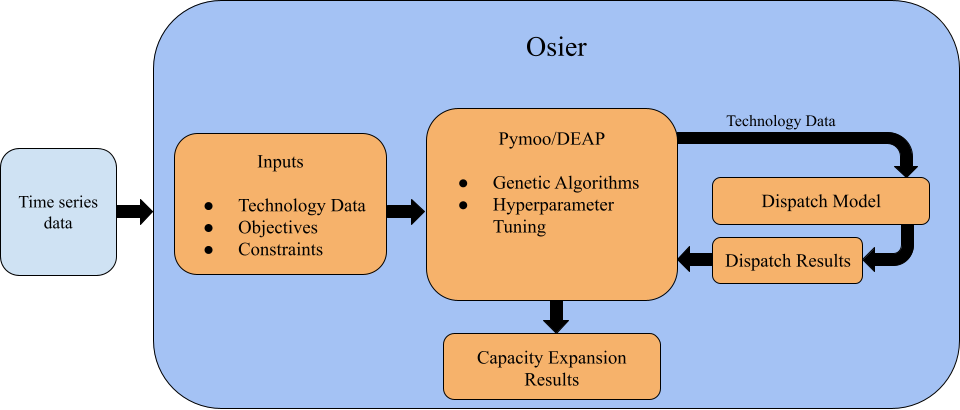
\includegraphics[width=\columnwidth]{figures/osier_flow}
    \caption{The flow of data into and within \ac{osier}}
    \label{fig:osier_flow}
\end{figure}

Technology data, objectives, constraints, and a dispatch model are all features
within \ac{osier}, while \ac{pymoo} drives the optimization of these objectives \cite{blank_pymoo_2020}.
The dispatch model is independently executable for inspecting specific test
cases and mapping solutions from other solvers onto \ac{osier}'s objective
space. The next sections elaborate on model inputs, \acfp{ga}, and the dispatch model's 
formulation.

% \textcolor{red}{This chapter is mostly written but there are a few things that
% should be added.}

\section{Inputs}

% \textcolor{red}{General thoughts:}

% Accurate input data are essential but curating data represents a challenging step in the
% modeling process. \ac{osier} attempts to lower this barrier by providing a
% variety of technology data from ``reliable'' sources.

% This section connects to the normative and descriptive portions of modeling. 

This section describes the input data and parameters that users must provide to run an \ac{osier} simulation. Broadly, \ac{osier} needs
technology data and some objectives to optimize. 

\subsection{Technology Data}
\ac{osier} only requires marginal costs and technology names in order to run successfully.
These data are needed to run the dispatch model. \ac{osier} also accepts operational data, such
as ramp rates and storage capacities. Additionally, \ac{osier} will understand any bespoke 
piece of data (e.g., ``popularity,'' ``technology-readiness score,'' or anything else) that
might be needed for a user-defined objective. All of these data are passed to \ac{osier}
through an \texttt{osier.Technology} object. Code listing \ref{listing:user-defined-technologies}
shows how users can create a simple technology object.

\begin{listing}[!ht]
    \caption{A basic technology object in \ac{osier}.}
    \label{listing:user-defined-technologies}
    \begin{minted}
    [ frame=lines, framesep=2mm, baselinestretch=1.2, bgcolor=LightGray,
    fontsize=\footnotesize, linenos ] {python} 
    from osier import ThermalTechnology

    fusion = ThermalTechnology(technology_name="Fusion",
                               dispatchable=True,
                               renewable=False,
                               fuel_cost=10*(GWh)**-1,
                               lifecycle_co2_rate=0.0,
                               )
    \end{minted}
    \end{listing}

\subsection{Objectives}
\label{section:osier_objectives}

There are many possible objectives to optimize. This section summarizes a few of
them and how they may be calculated in \ac{osier}. Due to \ac{pymoo}'s
structure, all objectives are minimized. Therefore, if users wish to maximize
some quantity, it must be reformatted with a reversal in sign to be an equivalent minimization objective.

\subsubsection{Per-unit-capacity}

Some quantities of interest depend on the \textit{capacity} of each technology.
For example, land use of different energy producers is often reported as a land
density $\text{km}^2/\text{MW}$. A generalized specific \textit{density} with respect to power 
may be $\text{unit}/\text{MW}$. The objective function for these quantities reads
\begin{align}
    \mathcal{K} &= \sum_g^G \textbf{CAP}_g \kappa_g ,
    \intertext{Where}
    \kappa &= \text{the power density of the \textit{g-th} technology} \quad \left[\frac{-}{MW}\right].
\end{align}

Table \ref{tab:objectives-per-capacity} lists some example objectives that could be
minimized or maximized.

\begin{table}[h]
    \centering
    \caption{Example objectives on a per-unit-capacity basis.}
    \begin{tabular}{cc}
       \toprule
       Quantity  & Units (per MW)\\
       \midrule
        Land Use & $\left[\text{km$^2$}\right]$\\
        Employment & $\left[\text{jobs}\right]$\\
        Capital Cost & $\left[\text{\$}\right]$\\
        Fixed O\&M Cost & $\left[\text{\$ / year}\right]$\\
        \bottomrule
    \end{tabular}
    \label{tab:objectives-per-capacity}
\end{table}

\subsubsection{Per-unit-energy}

Some quantities of interest depend on the \textit{amount of energy produced} by
each technology. For example, carbon emissions only occur when a coal or natural
gas plant burns fuel. A generalized specific \textit{intensity} with respect to energy 
may be in $\text{unit}/\text{MWh}$. The objective function for these quantities reads
\begin{align}
    \mathcal{E} &= \sum_g^G \xi_g \sum_t^T x_{g,t},
    \intertext{where}
    \xi_g &= \text{the energy density of the \textit{g-th} technology}\quad
    \left[\frac{-}{MWh}\right].
\end{align}

\begin{table}[h]
    \centering
    \caption{Example objectives on a per-unit-energy basis.}
    \begin{tabular}{cc}
       \toprule
       Quantity  & Units (per MWh)\\
       \midrule
        \acs{ghg} Emissions & $\left[\text{kg}\right]$ \\
        Water Use & $\left[\text{L}\right]$\\
        ``Safety'' & $\left[\text{deaths}\right]$\\
        Fuel Cost & $\left[\text{\$}\right]$\\
        Variable O\&M Cost & $\left[\text{\$}\right]$\\
        \bottomrule
    \end{tabular}
    \label{tab:objectives-per-energy}
\end{table}

\subsubsection{Reliability and Predictability}

Reliability has many definitions in the literature and it also depends heavily
on the dispatch method. A hierarchical flow, which dispatches energy based on a
set of rules (as opposed to true cost minimization), may simply report the
fraction of hours when electricity demand was not met by the model
\cite{donado_hyres_2020,bilil_multiobjective_2014,kamjoo_multi-objective_2016,riou_multi-objective_2021}.
\acs{lp} or \acs{milp} formulations typically have an energy balance constraint requiring 
electricity demand to be satisfied at all times, or within some specified tolerance. 
Thus reliability may be translated into a cost by determining consumers'
\ac{wtp} for electricity \cite{gorman_quest_2022, najafi_value_2021}. However,
this thesis relates system reliability to price volatility and net demand
predictability. Since the price of electricity is determined by matching supply
and demand, the price will spike when supply and demand are out of phase. For
instance, geopolitics may cause the supply of natural gas to drop, increasing
the spot price of electricity. Or, more commonly, the availability of solar and
wind resources may fall unexpectedly, leading to a greater demand for backup
energy. Both of those examples are difficult to predict; otherwise, fuel
reserves could be deployed, avoiding the price shock. Thus, I propose that
measuring the predictability and volatility of an energy system is an
appropriate proxy for reliability. Additionally, minimal price volatility is
considered an aspect of energy justice \cite{sovacool_energy_2015,
van_uffelen_revisiting_2022}.

In this thesis, I measure the  predictability of hourly electricity prices and
net demand using a measure from complexity science, \ac{wpe}
\cite{fadlallah_weighted-permutation_2013}. Permutation entropy, the precursor
to \ac{wpe}, is essentially the Shannon entropy for particular sequences of
values called \textit{motifs} \cite{bandt_permutation_2002}. \ac{wpe} expands on this
concept by weighting each instance of a motif by its variance
\cite{fadlallah_weighted-permutation_2013,garland_model-free_2014}. \ac{wpe} is
defined as
\begin{align}
    H_w(m) &= -\sum_{\pi \in \Pi} P_w(\pi)\log_2(P_w(\pi))
    \intertext{where}
    \pi &= \text{a particular motif,}\nonumber\\
    P_w &= \text{the probability of a given motif, $\pi$,}\nonumber\\
    &= \frac{\mathlarger{\sum\limits_{j\leq N}} w\left(x_j^{(m, \tau)}\right)\cdot\delta\left(\phi\left(x_j^{(m, \tau)}\right), \pi_i\right)}{\mathlarger{\sum\limits_{j\leq N}} w\left(x_j^{(m, \tau)}\right)}
    \intertext{and}
    w\left(x_j^{(m, \tau)}\right) &= \text{the weight of a particular vector}\nonumber\\
      &= \frac{1}{m}{\sum_{j}^m} \left(x_j^{(m,\tau)} - \Bar{x}\right)^2,\\\
     \phi(\cdot) &= \text{the ordinal pattern of a vector,}\nonumber\\
     \delta(\cdot) &= \text{Kronecker delta,}\nonumber\\
     m &= \text{the embedding dimension,}\nonumber\\
     \tau &= \text{the time delay}\nonumber.
\end{align}

There are other reliability metrics in the literature, frequently employing some
variation on the ``spread'' of data through standard deviation  or mean squared
error \cite{galvani_optimal_2021, galvani_unified_2014,
delsole_predictability_2004}. However, these metrics are unbounded and do not
contain any information about the underlying dynamics that produce a certain
distribution. Whereas \ac{wpe} can indicate a theoretical ceiling on
predictability \cite{garland_model-free_2014}. Importantly, \ac{wpe} works for
systems where the underlying dynamics are unknown. The Hurst exponent is another
measure of predictability, but it too has drawbacks, such as computational
expense and a stationarity requirement \cite{mesa_hurst_1993,
chandrasekaran_investigation_2019}. This thesis uses the \ac{wpe} implementation
I contributed to the open source package \texttt{PyEntropy}
\cite{donets_pyentropy_2023}.

\subsubsection{User-defined Objectives}

A key feature of \ac{osier} is the ability for users to define their own
objectives relatively easily. This feature is required
because modelers cannot know \textit{a priori} every objective that users might
be interested in optimizing. While \ac{osier} ships with some standard objective
functions, allowing users to create their own objectives makes every model
bespoke. With requisite user-supplied data \textit{any quantitative metric may be used as an objective in
\ac{osier}.} Every objective function has at least two arguments, the list of
technologies used in the model and the solved dispatch model. Users will never
have to pass these arguments manually since \ac{osier} will automatically call
the function during a simulation. One example of a user-defined objective might
be technology readiness. This objective is independent from the energy produced
and could be weighted by the capacity but is not a per-unit-capacity objective.
The values of the readiness parameter must be passed to each \texttt{Technology}
object, which can be accessed at run-time. Code listing
\ref{listing:user-defined-objective} shows the basic approach to creating a new
objective. 

\begin{listing}[!ht]
\caption{The fundamental way to create a novel objective in \ac{osier}.}
\label{listing:user-defined-objective}
\begin{minted}
[ frame=lines, framesep=2mm, baselinestretch=1.2, bgcolor=LightGray,
fontsize=\footnotesize, linenos ] {python} 

nuclear.readiness = 9
fusion.readiness = 3

technology_list = [nuclear, fusion]

def osier_objective(technology_list, solved_dispatch_model): 
    """ 
        Calculate the capacity-weighted technology readiness 
        score for this energy mix. 
    """

    total_capacity = np.array([t.capacity for t in technology_list]).sum()
    
    objective_value = np.array([t.readiness*t.capacity 
                                for t in technology_list]).sum()

    return objective_value / total_capacity
\end{minted}
\end{listing}
\noindent
Importantly, because all technologies in \ac{osier} are Python objects, users
can add attributes at will. Such as the technology readiness level as shown in
Code listing \ref{listing:user-defined-objective}. 

\subsection{Constraints}
\label{section:constraints}

Besides the physical constraints defined in Section \ref{section:dispatch_model},
\ac{osier} does not have any default constraints. This is because each
additional constraint corresponds to an additional assumption and will affect
the trade-off analysis that makes \ac{moo} so powerful. However, there are some
circumstances where the optimal solutions are still
infeasible in practice. For instance, if a community wants to determine the best
energy mix according to their unique objectives, this community might not have
the budget for even a least-cost solution because the capital requirements are
too high. Therefore, they must constrain the capital cost for their modeling
problem. Thus, \ac{osier} enables the following:
\begin{enumerate}
    \item Users may define their own constraints.
    \item Any objective function may be transformed into a constraint.
\end{enumerate}
This feature makes \ac{osier} unique among \acp{esom}.
Single-objective \acp{esom} can never account for unique situations such as the
one suggested above, nor any other bespoke considerations. In the case above,
the capital cost may constrain the problem while still minimizing the total
cost. The solutions under these conditions will have a higher total cost but
could be achievable in the near term due to meeting capital cost requirements.
\section{Genetic Algorithms}
\label{section:genetic-algorithms}

Rather than rely on \ac{lp} to model future capacity requirements, in this
thesis, \acp{ga} assume the role of investment optimizer. \acp{ga} share a
fundamental algorithmic structure, which is \cite{blank_pymoo_2020}
\begin{enumerate}
    \item \textbf{Initialize} a starting population of $N_p$ individuals, where
    each individual has a set of ``genes'' that are randomly chosen from the
    bounds of the decision variables.
    \item Each individual in the population is \textbf{evaluated} for
    ``fitness.'' 
    \item The \textbf{fittest}, $N_f$ individuals ``survive'' and persist in the
    next generation.
    \item A ``selection'' operator \textbf{chooses} among the surviving
    individuals to mate.
    \item The parents are \textbf{combined} using a ``crossover'' operator,
    thereby filling the remaining $N_p - N_f$ individuals for the next
    generation.
    \item The offspring are finally \textbf{mutated} with some probability,
    $\mu$, to improve genetic diversity.
\end{enumerate}
\noindent
Figure \ref{fig:genetic-alg} illustrates the flow of these steps applied to an
energy systems model.

\begin{figure}[ht]
        \centering
        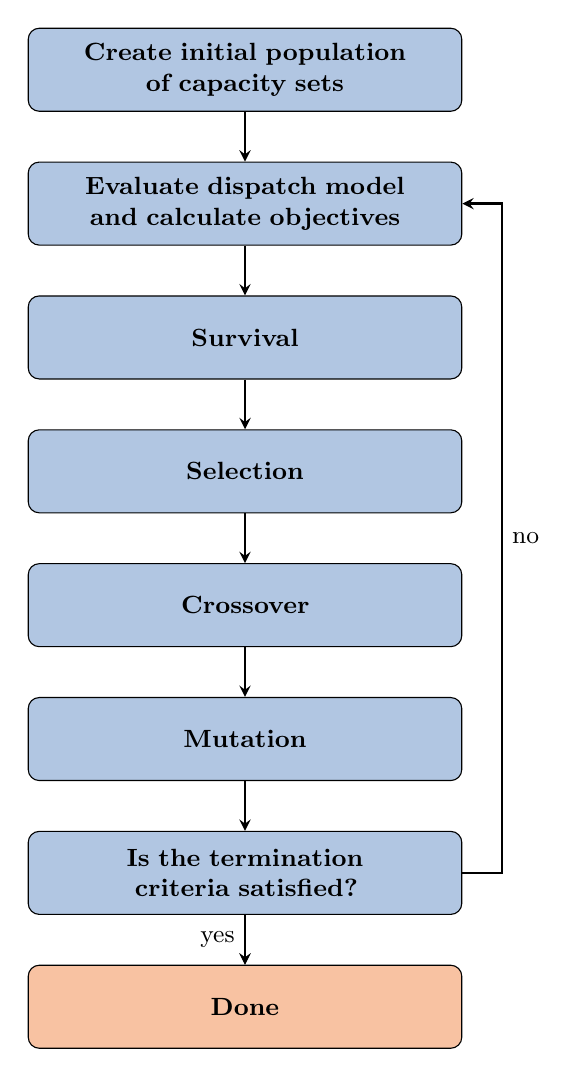
\begin{tikzpicture}[node distance=1.7cm]
                \tikzstyle{every node}=[font=\small] \node (1) [lbblock]
                {\textbf{Create initial population\\ of capacity sets}}; \node
                (2) [lbblock, below of=1] {\textbf{Evaluate dispatch model and
                calculate objectives}}; \node (3) [lbblock, below of=2]
                {\textbf{Survival}}; \node (4) [lbblock, below of=3]
                {\textbf{Selection}}; \node (5) [lbblock, below of=4]
                {\textbf{Crossover}}; \node (6) [lbblock, below of=5]
                {\textbf{Mutation}}; \node (7) [lbblock, below of=6] {\textbf{Is
                the termination \\ criteria satisfied?}}; \node (8) [loblock,
                below of=7] {\textbf{Done}}; \draw [arrow] (1) -- (2); \draw
                [arrow] (2) -- (3); \draw [arrow] (3) -- (4); \draw [arrow] (4)
                -- (5); \draw [arrow] (5) -- (6); \draw [arrow] (6) -- (7);
                \draw [arrow] (7) -- (8); \draw [arrow] (7) -- node[anchor=east]
                {yes} (8); \draw [arrow] (7) -- ([shift={(0.5cm,0cm)}]7.east)--
                node[anchor=west] {no} ([shift={(0.5cm,0cm)}]2.east)--(2);
        \end{tikzpicture}
        \caption{The basic flow of the \ac{ga} used in this thesis.}
        \label{fig:genetic-alg}
\end{figure}

\subsection{Specific \Aclp{ga}} The variety of \acp{ga} comes from different
types of operators being applied to the selection, crossover, and mutation
steps. Section \ref{section:moo-in-energy} showed that \ac{nsga2} is a popular
genetic algorithm choice. However, this algorithm performs poorly with greater
than three objectives \cite{deb_fast_2002, seada_unified_2016}. This thesis
uses a more modern algorithm, \ac{unsga3}. \ac{unsga3} builds on its
predecessors \ac{nsga2} and \ac{nsga3} by unifying efficient solutions of mono-,
multi-, and many-objective problems in a single algorithm.


\ac{nsga2} improves on the basic \ac{ga} by introducing a more sophisticated
mating and selection algorithms. Instead of random selection, the individuals
are sorted by rank (i.e. fitness) and crowding distance in binary tournament
mating selection. The crowding distance is simply the Manhattan distance between
individuals. A greater crowding distance is desirable to preserve diversity and
since the extreme points are maximally diverse they should always persist and
are therefore assigned a crowding distance of infinity \cite{deb_fast_2002}.

The successor to \ac{nsga2}, \ac{nsga3}, enhances the many-objective
capabilities of the former by introducing reference directions. Reference
directions are used for initialization and the survival steps. In addition to
fitness, individuals are chosen based on their proximity to a reference line,
thus ensuring population diversity which greatly important for many-objective
problems. Since diversity is handled by reference directions, individuals are
selected randomly for mating. References directions are rays passing through
uniformly spaced points on the unit simplex \cite{seada_unified_2016,
blank_generating_2021}. In this thesis, I use the Riesz s- Energy method
described by Blank et al. to calculate these points for a problem with an
arbitrary number of objectives \cite{blank_generating_2021}. Figure
\ref{fig:ref-dirs} illustrates a set of initialized reference directions used
in such methods.

\begin{figure}[h]
  \centering
  \resizebox{0.6\columnwidth}{!}{\input{figures/reference_directions.pgf}}
  \caption{A set of reference directions for a three-objective problem.}
  \label{fig:ref-dirs}
\end{figure}

\ac{nsga2} is useful for mono- and multi-objective functions while \ac{nsga3} is
better for many-objective problems. \ac{unsga3} can handle any number of
objectives by introducing the binary tournament from \ac{nsga2} and reducing to
the most efficient algorithm for the problem at hand \cite{seada_unified_2016}.
Chapter \ref{chapter:benchmark-results} demonstrates these three algorithms in 
Section \ref{section:4-exercise-1}.

\subsection{Hyperparameter Tuning}
Similar to other machine learning models, \acp{ga} have several hyperparameters
that must be tuned for optimal behavior. These hyperparameters include
probabilities for mutation, crossover, and selection, as well as the number of
parents, number of offspring, and population size. Determining ideal
hyperparameters is often performed using either a grid search or random sampling
\cite{bergstra_random_2012}. This thesis adopts the approach from Blank and Deb
\cite{blank_pymoo_2020} using a genetic algorithm to identify the ideal
hyperparameters. A multi-objective problem is converted into a single objective problem 
by choosing one objective and optimized with the target \ac{ga}, then a second \ac{ga} 
drives a new problem where the decision variables are hyperparameters of the desired algorithm.

\subsection{Convergence}
There are several ways to stop a simulation in \ac{pymoo}. A simulation may end
after reaching
\begin{enumerate}
    \item a specified end time (e.g., 100 minutes),
    \label{it:convergence1}
    \item a specified number of evaluations or iterations (e.g., 500 individual
    evaluations or 20 generations),
    \label{it:convergence2}
    \item a tolerance value in the design space,
    \label{it:convergence3}    
    \item a tolerance value in the objective space.
    \label{it:convergence4}
\end{enumerate}

It is possible that criteria \ref{it:convergence3} and \ref{it:convergence4}
will never be met; therefore, they are often combined with either of the first
two criteria. The fourth convergence criterion is the most interesting due to
the challenge of calculating an appropriate metric. This thesis uses the weakly
Pareto-compliant algorithm \ac{igdp} over the more common hypervolume
calculation due to its reduced computational requirements
\cite{ishibuchi_modified_2015}.

\subsection{\acs{pymoo} and \acs{deap}}

The \ac{esom} framework developed in this thesis is built on top of \ac{pymoo}
and \ac{deap}. \ac{pymoo} is an open-source library for \acp{ga} developed by
the creators of \ac{nsga2} and \ac{unsga3} \cite{blank_pymoo_2020}. This package
implements several \acp{ga} out-of-the-box and offers a set of visualization
tools and hyperparameter tuning. \ac{deap} is another open-source library
offering a toolkit for constructing \acp{ga} and therefore has fewer prepackaged
algorithms than \ac{pymoo}. There are robust reasons to use both libraries, so
\ac{osier} facilitates both. \ac{pymoo} provides a broader range of tools 
while \ac{deap} enables greater flexibility with \ac{ga} implementation and more
straightforward procedures for stopping a simulation and restarting at a later
time.





\section{Dispatch Model}
\ac{osier} offers three models for dispatching energy. The first is a merit order
dispatch model that optimally dispatches electricity according to the marginal
cost of generation with perfect foresight. This model is formulated as a
\acf{lp} and written in \ac{pyomo}. Similarly, the second dispatch model follows
merit-order but electricity is dispatched according to a hierarchy of rules and
is myopic. This approach is advantageous over the \ac{lp} formulation because it
facilitates parallelization and doesn't have the overhead cost of setting up the
problem. However, dispatch solutions may be sub-optimal compared to the \ac{lp}
approach. The third model is a simplified dispatch model that is very fast,
taking advantage of vectorization, but makes several assumptions about the
energy system and is not appropriate for general use.

\subsection{Economic/Merit-order dispatch}
\label{section:merit_order}

 The economic dispatch model minimizes the generation cost subject to physical
 constraints but does not optimize capacity investments. The complete set of
 equations for the model is detailed below.
\begin{align}
    \intertext{Minimize: }
    \label{eq:dispatch-objective}
    &\left(\sum_t^T\sum_g^G \left[C_{g,t}^{fuel} + C_{g,t}^{vom}\right]x_{g,t}
    \right)+\left(\sum_t^T\sum_g^S x_{g,t}c_{g,t}\pi\right)\\
    \intertext{such that,}
    \intertext{1. The generation meets demand, less the amount of energy stored or curtailed, 
    within a user-specified tolerance (undersupply and oversupply),}
    \left[\sum_g^Gx_{g,t}-\sum_g^S c_{g,t}\right] &\geq \left(1-\text{undersupply}\right)\text{D}_t\quad \forall \quad t \in T, S, \\
    \left[\sum_g^Gx_{g,t}-\sum_g^S c_{g,t}\right] &\leq \left(1+\text{oversupply}\right)\text{D}_t \quad \forall \quad t \in T, S,
    \intertext{2. A generator's production, $x_{g}$ does not exceed its capacity at any time, $t$}
    x_{g,t} &\leq \textbf{CAP}_{g}\Delta \tau \quad \forall \quad g,t \in G,T
    \intertext{3. A generator's ramping rate is never exceeded,}
    \frac{x_{r,t} - x_{r,t-1}}{\Delta \tau} = \Delta P_{r,t} &\leq
        \rho^{up}_g\textbf{CAP}_g\Delta\tau \quad \forall \quad r,t
        \in R, T,\\
    \frac{x_{r,t} - x_{r,t-1}}{\Delta \tau} = \Delta P_{r,t} &\leq
        -\rho^{down}_g\textbf{CAP}_g\Delta\tau \quad \forall \quad r,t
        \in R, T,
    \intertext{4. Storage capacity for each storage technology is never exceeded}
    \textbf{SOC}_{s,t} &\leq \textbf{CAP}^S_{s} \quad \forall \quad s,t \in S,T,
    \intertext{5. Storage discharge cannot exceed stored energy.}
    x_{s,t} &\leq \textbf{SOC}_{s,t} \quad \forall \quad s,t \in S,T,
    \intertext{6. Storage charge rate cannot exceed unit capacity}
    c_{s,t} &\leq \textbf{CAP}_{s}\Delta \tau \quad \forall \quad s,t \in S,T,
    \intertext{where,}
    G &= \text{ the set of all generating technologies},\nonumber\\
    R &= \text{ the set of all ramping technologies}, \quad R \subset G,\nonumber\\
    S &= \text{ the set of all storage technologies}, \quad S \subset G,\nonumber\\
    T &= \text{ the set of all time periods in the model},\nonumber\\
    D_t &= \text{ the demand at each time period, \textit{t}},\nonumber\\
    \textbf{CAP}_g &= \text{ the capacity of the \textit{g-th} technology}\quad \left[MW\right],\nonumber\\
    \textbf{CAP}^S_g &= \text{ the storage capacity of the \textit{g-th} technology}\quad \left[MWh\right],\nonumber\\
    \textbf{SOC}_{s,t} &= \text{ the state of charge of the \textit{g-th} technology at time \textit{t}}\quad \left[MWh\right]\nonumber,\\
    \Delta\tau &= t_{i+1} - t_i \quad \forall \quad t_i \in T \quad \left[h\right],\nonumber\\
    x_{g,t} &= \text{ the energy produced by generator, \textit{g}, at time, \textit{t}}\quad \left[MWh\right]\nonumber,\\
    c_{s,t} &= \text{ the energy stored by storage technology, \textit{s}, at time, \textit{t}}\quad \left[MWh\right]\nonumber,\\
    \rho_g &= \text{ the up/down ramp rate for technology, \textit{g}} \quad \left[-\right]\nonumber,\\
    \pi &= \text{ A small penalty for simultaneous charging and discharging.}\nonumber
\end{align}
The second term in the objective function, Equation \ref{eq:dispatch-objective},
represents a minor penalty to prevent the unphysical behavior of simultaneous
charging and discharging from storage technologies. I used this approach because
constraining this behavior requires a binary variable that makes the problem
non-convex and therefore requires a more sophisticated solver. A small but
sufficiently large $\pi$ will always nullify the penalty term. This dispatch
model reflects the minimum physical constraints for an energy system without
considering fine-scale operational details such as frequency control. Equation
\ref{eq:dispatch-objective} assumes that the retail cost for generating
electricity is identical to the marginal cost of producing electricity. 

\subsection{Hierarchical dispatch}

\subsection{Simplified dispatch}
\section{\acs{mga} with \acl{moo}}
\label{section:mga-moo}

\textcolor{red}{This section talks about handling ``structural uncertainty'' with \ac{osier}.}


This thesis applies some ideas from \ac{mga} to the analysis of the sub-optimal
space from a \acl{moo} problem. Due to their iterative process, \acp{ga}
naturally generate many samples in a problem's feasible space. However, this
does not lead to a ``limited set'' of solutions but rather a potentially
infinite set. Some literature developed \acp{ga} that directly use \ac{mga} in
the iterative process
\cite{zechman_evolutionary_2004,zechman_evolutionary_2013}. However, existing
Python libraries such as \ac{pymoo} and \ac{deap} do not implement these
methods, and the challenge is not an inability to sample the sub-optimal space,
but rather to provide a comprehensible subset of solutions. The algorithm I
developed in this thesis to search the near-feasible space is the following:

\begin{enumerate}
    \item Obtain a set of Pareto-optimal solutions \textit{using any \ac{ga}}.
    \item Decide on a slack value (e.g., 10\% or 0.1), which represents an
    acceptable deviation from the Pareto front.
    \item Create a ``near-feasible front'' where the coordinates of each point
    are multiplied by unity plus the slack value. This is equivalent to relaxing
    the objective functions and converting them to a constraint. 
    \item Every individual is checked if all of its coordinates are
    \begin{itemize}
        \item below all of the coordinates for at least one point on the
        near-feasible front and
        \item above all of the coordinates for at least one point on the Pareto
        front.
    \end{itemize}  
    \item Lastly, the set of interior points may be sampled either randomly or with a
    farthest-first-traversal algorithm to restrict the number of analyzed solutions.
\end{enumerate}
\noindent
Figure \ref{fig:nd-mga} and Figure \ref{fig:3d-mga} demonstrate this algorithm
with 10 percent slack for a 2-D and 3-D Pareto front, respectively. Figure
\ref{fig:nd-mga} shows clearly that only points within the near-optimal space
(gray) are considered. Illustrating this behavior in three dimensions (and
above) is considerably more difficult. The 3-D interior points should be covered
by both surfaces, obstructing their view. Figure \ref{fig:3d-mga} shows that
this is the case in three panels. First, a top view of an opaque Pareto front
(green) where no interior points can be observed. Second, the same view with a
translucent Pareto front, revealing interior points and the near-optimal front
(blue). Finally, the view from underneath the near-optimal front once again
obscures the interior points, except for two near the edges of the sub-optimal
space. The tested points are omitted for clarity.
 

\begin{figure}[h]
  \centering
  \resizebox{0.6\columnwidth}{!}{\input{figures/nd-mga-paretofront.pgf}}
  \caption{All of the alternative points inside the near-feasible space selected
  using the algorithm described in Section \ref{section:mga-moo}.}
  \label{fig:nd-mga}
\end{figure}

\begin{figure}[H]
  \centering
  \resizebox{1\columnwidth}{!}{\input{figures/3d-mga-paretofront.pgf}}
  \caption{From left to right: An opaque Pareto front; a translucent Pareto front showing the interior points above a sub-optimal front; and the sub-optimal front hiding the interior points from a different angle.}
  \label{fig:3d-mga}
\end{figure}
\section{Limitations of \ac{osier}}

This section describes some of the limitations in \ac{osier}'s modeling details
and scope. For example, \ac{osier} does not model interactions between the
environment and the energy system. It also does not include a way to model the
effect of carbon emissions and/or any kind of climate forcing from heat-trapping
emissions nor any kind of geoengineering measures.

This responds to some of Cliff's comments on \ac{osier}.


\chapter{Benchmark Results}
\label{chapter:benchmark-results}

% \textcolor{red}{This chapter will remain largely unchanged except for maybe one
% additional example, demonstrating a different dispatch model that is much faster
% but less robust. This new dispatch model will be used in the following chapter
% where I investigate further examples including a hypothetical ``data center''
% and an improvement on the \acf{set} \cite{wigeland_nuclear_2014}.}

% \section{Exercise 0: Demonstrating \ac{osier}}
% \textcolor{red}{This section is new in the dissertation!}

% This section demonstrates some of the basic features of Osier. This section should be based 
% on the examples in \ac{osier}'s documentation.

% \section{Exercise 1: Deciding Among Evolutionary Algorithms}

% \textit{Already written in prelim document.}

% \section{Exercise 2: Exploring objective space}

% \textit{Already written in prelim document.}

% \section{Exercise 3: Four Simultaneous Objectives}

% \textit{Already written in prelim document.}

% \section{Exercise 4: Validating a Simplified Approach}

% \textcolor{red}{This section is new in the dissertation.}

\chapter{Examples with \acs{osier}}
\label{chapter:examples}

\textcolor{red}{This chapter is entirely new to this thesis!}

\section{Example 1: Updating the \ac{set}}

\textcolor{red}{Points to hit:}
\begin{enumerate}
    \item Addressing the climate crisis requires new infrastructure and new energy sources.
    \item Progress has been stifled on many fronts, not the least of which has been public opposition to energy projects. Including wind, solar, and nuclear.
    \item Some of this opposition results from dissatisfaction with process.
    \item Opposition can be pre-empted with sincere and proactive community engagement.
    \item In the case of nuclear energy, some of these efforts are already underway with concepts such as consent-based siting entering the nuclear zeitgeist.
    \item ???
    \item Introduce the \ac{set} tool
    \item  Introduce \ac{osier} as a tool for multi-objective optimization.
\end{enumerate}

\textcolor{red}{Benefits of using \ac{osier}}:
\begin{enumerate}
    \item Python interface allows direct coupling with external models and data sources for greater flexibility.
    \item Enables, but does not require, a weighting scheme for decision making.
    \item Allows users to analyze tradeoffs among competing objectives.
    \item Allows users to compare lifecycle impacts with non-nuclear technologies.
    \item Can flexibly add additional assessment criteria (e.g., Energy return on investment). 
\end{enumerate}

\textcolor{red}{Results}
\begin{enumerate}
    \item Does using \ac{osier} support the previous conclusions about the most promising evaluation groups?
\end{enumerate}

\subsection{Overview of the Nuclear Fuel Cycle}

\subsection{What is the \ac{set}?}

\subsection{What metrics are available?}

\subsection{Data for the simulation}

\subsection{Results}

\subsection{Discussion}

% \section{Example 2: Powering a Data Center}

% \subsection{Why data centers?}

% \subsection{What technology options exist?}

% \subsection{Data for the simulation}

% \subsection{Results}

% \subsection{Discussion}


\chapter{Using modeling to enhance just outcomes}
\label{chapter:communities}
\iffalse


This chapter addresses my proposal to ``validate'' \ac{osier} by conducting a
case study of energy planning processes in Champaign-Urbana through interviews
with decision makers and planners about energy justice, energy modeling, and
energy planning. As well as introduce interviewees to \ac{osier} itself and
solicit feedback from them about its potential usefulness and what obstacles may
interfere with its adoption. 

Although I originally set out to conduct a limited case study of Chambana, I
discovered that municipalities in Illinois do not, in general, have the decision
making authority to make specific choices about their energy supply.
Thus, I expanded my study to the state level; interviewing people from the
\ac{ipa} and \ac{icc}. This expanded scope provided evidence for structural
challenges blocking municipal influence from energy planning processes. Further,
this evinces a tension among distributive, procedural, and recognition justice.

\section{Progress on developing tools for local use}

\begin{itemize}
    \item The literature review chapter indicated that most energy modeling tools
    and much of the related literature focus on state- or national-scale energy
    systems.
    \item The the hyper-local section highlighted some studies that integrated
    local perspectives with energy modeling. Those papers include 
    \cite{mckenna_combining_2018, johannsen_municipal_2023, fleischhacker_portfolio_2019}
    \item There have also been studies investigating the development of models for, and
    use by, city and urban planners.
\end{itemize}

\section{Municipal Levers: How municipalities make choices about their energy supply}
There are generally four ways municipalities can make choices about their energy supply.

\subsection{\ac{mca}}
This is where municipalities participate in electricity markets on behalf of
their residents. Although this allows municipalities to choose an energy supply
besides the standard portfolio provided by an electric utility, municipalities
do not have full control over their energy supply. Instead, municipalities
negotiate for a few portfolios through a bidding process. While they can specify
some criteria, such as a percentage of renewable energy, the specific generation
mix depends on the company that developed the portfolio bid. Further, residents
are still allowed to opt-out of \ac{mca} and elect the standard portfolio
provided by their electric utility.

\subsection{Utility ownership}
Some municipalities in Illinois, such as Naperville, own their own distribution
system. This gives a municipality greater control over the design of their
utility system and allows a municipality to make decisions about the tradeoff
between cost and resiliency. For example, Naperville undergounded most of the
electric distribution system and new distribution is automatically undergounded.
However, this model does not award control of electric supply to the
municipality, which must procure electricity through another entity such as the
\acf{imea}.

\subsection{Municipal-owned generation}
In very few cases, a municipality may own some of its own generation. \ac{uiuc}
owns a coal and natural gas plant, a solar array, chilled water storage, and
participates in a \ac{ppa} to purchase wind power. More commonly, municipalities
will lease land cheaply to a solar company, for example, and purchase some or all
of the rights to that electricity through a \ac{ppa}. 

\subsection{Municipal-owned buildings}

\fi

\chapter{Conclusions}



% per Graduate College preference, place the \appendix and the appendices content before the
% bibliography (here) only if the appendices contain references.

\backmatter

\printbibliography[heading=bibintoc,title={References}]

% the below lines are only needed if bibliography precedes appendices
% uses https://tex.stackexchange.com/a/440212 to continue page numbering
\clearpage
\setcounter{counterforappendices}{\value{page}}
\mainmatter
\setcounter{page}{\value{counterforappendices}}

\appendix

\chapter{Interview Guide}
\label{chapter:interview-guide}
This interview guide was used to structure the interviews as described in
Section \ref{section:interview-methods}.

\begin{enumerate}
    \item Background
    \begin{enumerate}
        \item What is your role at your organization/municipality?
        \item How are energy planning activities organized in your
        organization/municipality?
        \item What are your perceptions of these energy planning process?
        \item Who are the members/relevant stakeholders of your community?
    \end{enumerate}
    \item Understanding existing planning processes
    \begin{enumerate}
        \item What steps are taken in the process and what factors are
        considered?
        \item How often does your organization/community undergo an energy
        planning process?
        \item What is the final product?
        \item To my knowledge, the municipality/organization has the following
        sustainability/climate plans, do you have other energy-related plans?
        \item What methods or tools do you use for planning?
        \item How, if at all, are policy options quantified?
        \item What are the objectives or priorities for the resulting energy
        policy?
        \item How did your community/organization develop these priorities?
        \item Which stakeholders are involved internally or externally?
        \item What kinds of concerns do your
        [constituents/stakeholders/community members] have about energy in
        [municipality/constituency]?
        \item What does stakeholder engagement look like?
        \item What is the role of expert opinion in creating an energy vision?
        \item How does the energy planning process consider the impact on its
        neighbors?
        \item To what extent does your energy planning process consider impacts
        to other communities?
        \item Does your institution coordinate with other municipalities or
        communities?
    \end{enumerate}
    \item How is energy justice incorporated in planning processes?
    \begin{enumerate}
        \item Do you or your municipality explicitly consider justice or
        fairness during the planning process?
        \item Does your organization/municipality track outcomes related to
        energy burden within your community?
        \item Does your municipality track health/environmental/economic impacts
        from energy production within the community?
        \item What does a ``clean energy transition'' mean for you? For your
        community?
        \item What do you see as the role of [municipality/organization] in
        Illinois' clean energy transition?
        \item Are members of your community affected by the clean energy
        transition? Would you categorize these effects as benefits or burdens?
    \end{enumerate}
    \item How are energy models and results used to guide planning processes?
    \begin{enumerate}
        \item How does your community/organization use modeling software to
        support its vision, if at all?
        \item Are modeling results used during energy planning?
        \item Has your community collaborated with another organization to
        conduct energy modeling in the last five years?
    \end{enumerate}
    \item How could \ac{osier} be used to support energy planning processes?
    \begin{enumerate}
        \item Would your organization/municipality use this tool?
        \item If not this specific tool, is there a tool that exists/does not
        exist that is/would be useful?
        \item What changes would \ac{osier} need to adopt for it to be useful to
        you?
        \item How would employing this tool differ from existing strategies or
        processes?
        \item Would this tool be useful to facilitate dialogue between the
        public and decision-makers related to energy policies?
        \item What objectives do you think would be important to include in the
        model when desigining an energy vision for your community?
    \end{enumerate}
\end{enumerate}

\end{document}
